\documentclass{beamer}
\usepackage{algpseudocode}
\usepackage[utf8]{inputenc}
\usepackage{graphicx}
\usepackage{xcolor}
\usepackage{soul}
\usepackage{hyperref}

\usepackage{colortbl}

\usetheme{Antibes}
\usecolortheme{dolphin}

\usefonttheme[onlymath]{serif}

\definecolor{LightBlue}{RGB}{140,186,252}

\title{\textbf{Introduction to Deep Learning}}
\author{Distributed Lab}
\date{January 18, 2024}

\titlegraphic{
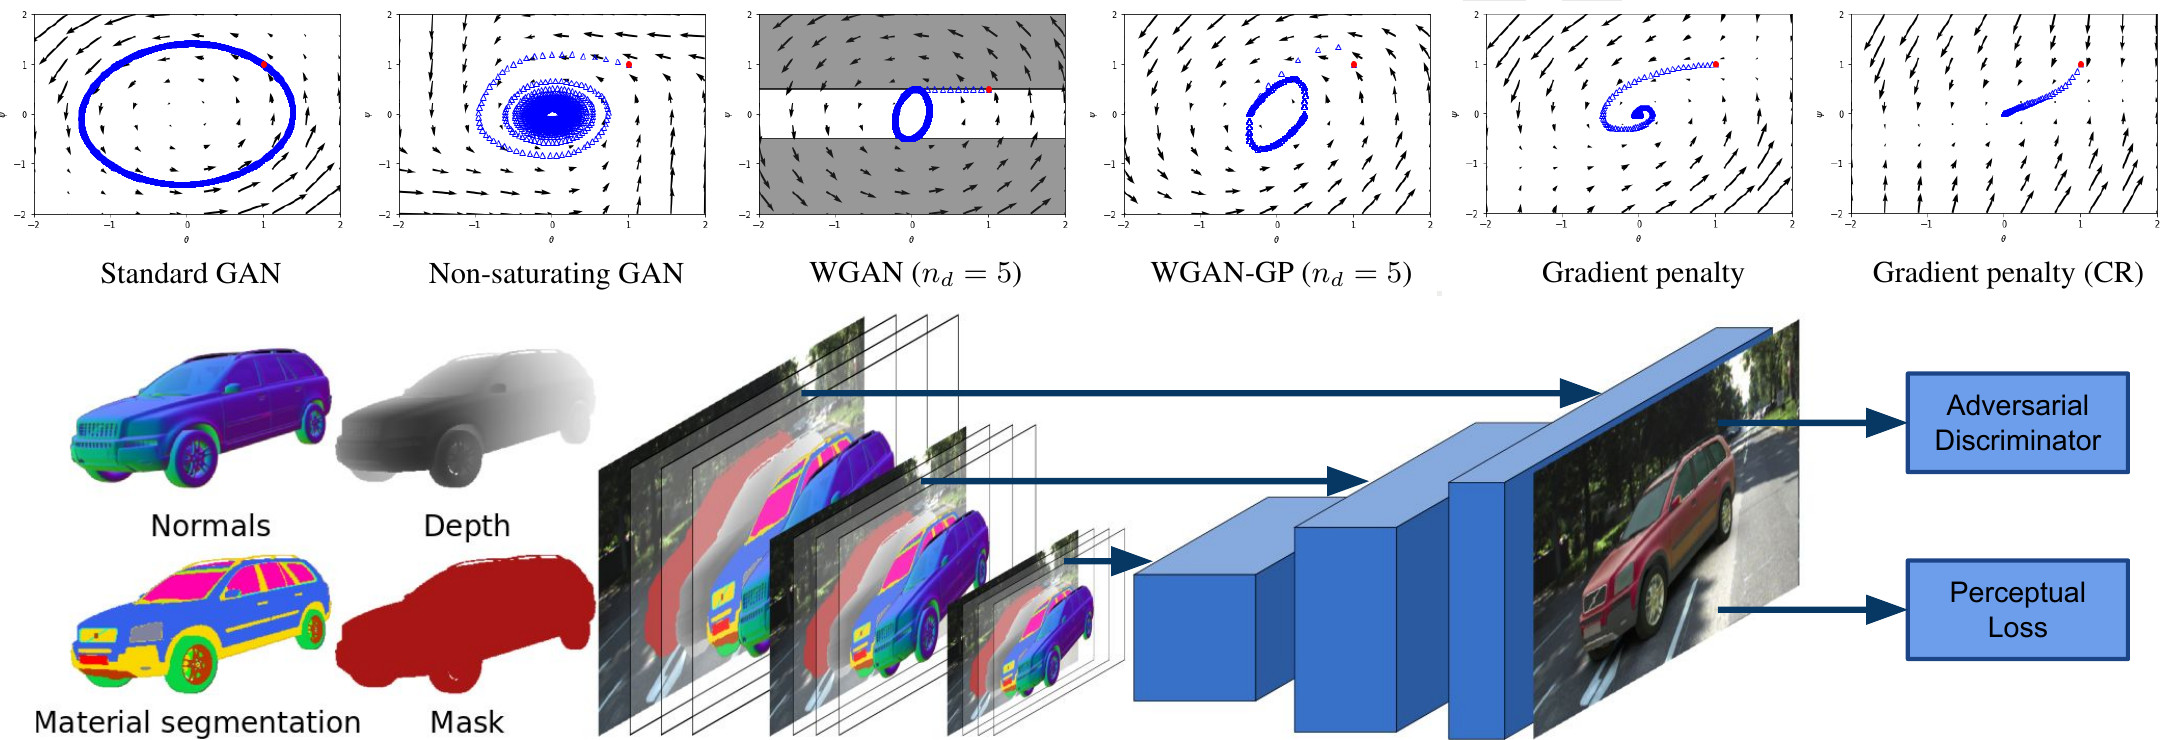
\includegraphics[width=0.9\textwidth]{images/presentation/neural.jpg}
}

\expandafter\def\expandafter\insertshorttitle\expandafter{%
  \insertshorttitle\hfill%
  \insertframenumber\,/\,\inserttotalframenumber}

\AtBeginSection[]{
  \begin{frame}
  \vfill
  \centering
  \begin{beamercolorbox}[sep=8pt,center,shadow=true,rounded=true]{title}
    \usebeamerfont{title}\insertsectionhead\par%
  \end{beamercolorbox}
  \vfill
  \end{frame}
}

\usepackage{algorithm}
\usepackage{algpseudocode}
\usepackage{listings}
\usepackage{xcolor}
\usepackage{dsfont}

\definecolor{codegreen}{rgb}{0,0.6,0}
\definecolor{codegray}{rgb}{0.5,0.5,0.5}
\definecolor{codepurple}{rgb}{0.58,0,0.82}
\definecolor{backcolour}{rgb}{0.95,0.95,0.92}

\lstdefinestyle{mystyle}{
    backgroundcolor=\color{backcolour},   
    commentstyle=\color{codegreen},
    keywordstyle=\color{magenta},
    numberstyle=\tiny\color{codegray},
    stringstyle=\color{codepurple},
    basicstyle=\ttfamily\footnotesize,
    breakatwhitespace=false,         
    breaklines=true,                 
    captionpos=b,                    
    keepspaces=true,                 
    numbers=left,                    
    numbersep=5pt,                  
    showspaces=false,                
    showstringspaces=false,
    showtabs=false,                  
    tabsize=2
}
\lstset{style=mystyle}

\begin{document}
	\frame {
		\titlepage
	}

    \frame {
        \frametitle{Spoiler}
        At the end of this lecture, we will build a digit recognition neural network!
        
        \begin{figure}
            \centering
            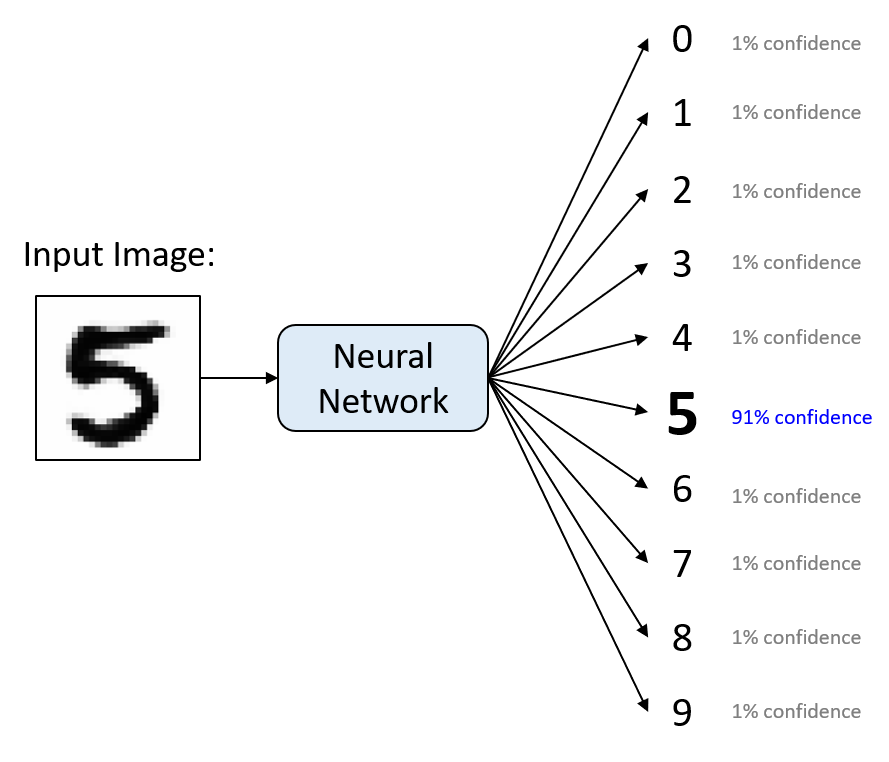
\includegraphics[width=0.6\textwidth]{images/presentation/digit_recognition.png}
        \end{figure}
    }
 
	\begin{frame}{Plan}
        \tableofcontents
    \end{frame}
	 
	\section{Introduction}
	\subsection{Why do we care?}
	\begin{frame}{Why do we care about Machine Learning?}		
		\begin{columns}
        % Description
        \begin{column}{0.5\textwidth}
            \begin{enumerate}
                \item Machine Learning becomes more and more used in many areas. Same might happen with blockchain and cryptography at some point.
                \item Deep Learning is extensively used in security systems.
                \item We have already encountered Deep Learning problems on ``certain'' projects.
                \item Machine Learning is fun!
            \end{enumerate}
        \end{column}
        % Column 2    
        \begin{column}{0.5\textwidth}
            \begin{figure}
            \centering
                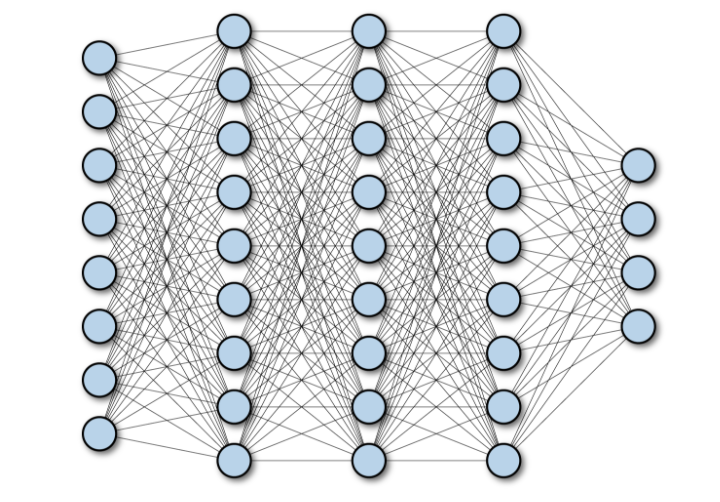
\includegraphics[width=1\textwidth]{images/presentation/web.png}
            \end{figure}
        \end{column}
        \end{columns}
	\end{frame}

    \begin{frame}{ML in Information Security: Liveness Detection}
	    \begin{figure}
        \centering
            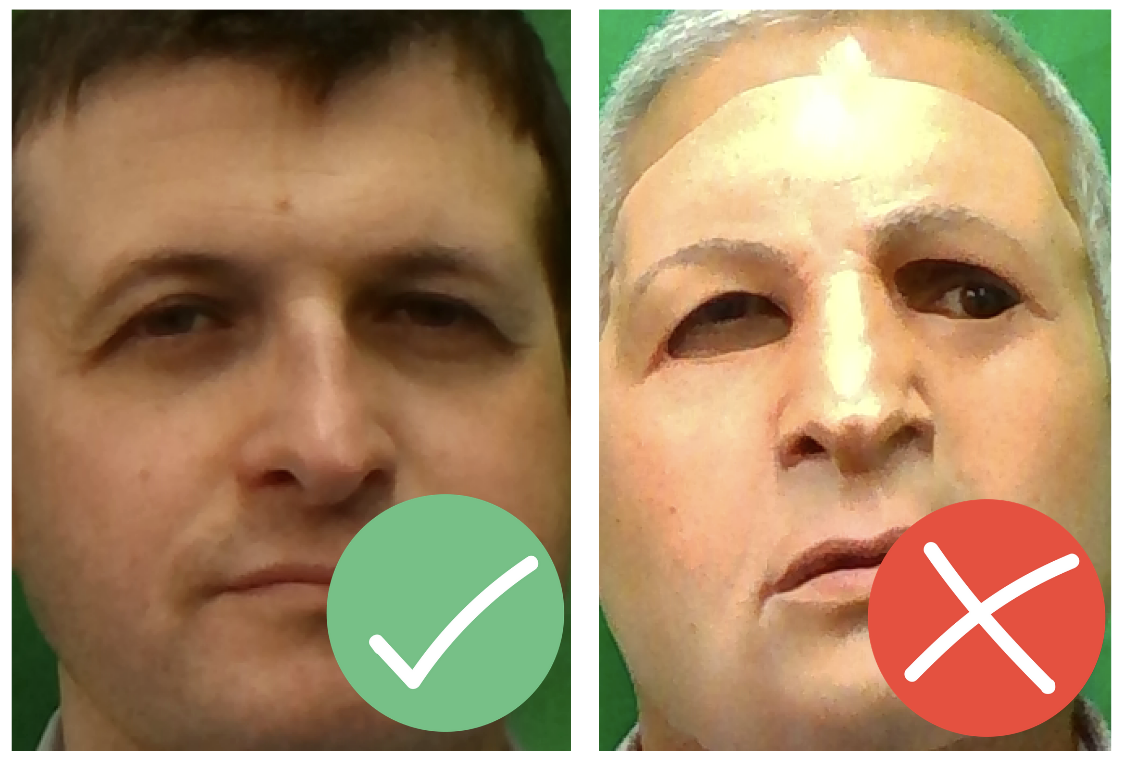
\includegraphics[width=0.7\textwidth]{images/presentation/statement.png}
            \caption{Liveness Detection. See our recently published paper: \href{https://ceur-ws.org/Vol-3608/paper19.pdf}{https://ceur-ws.org/Vol-3608/paper19.pdf}}
        \end{figure}
	\end{frame}

    \begin{frame}{ML in Information Security: Face Recognition}
	    \begin{figure}
        \centering
            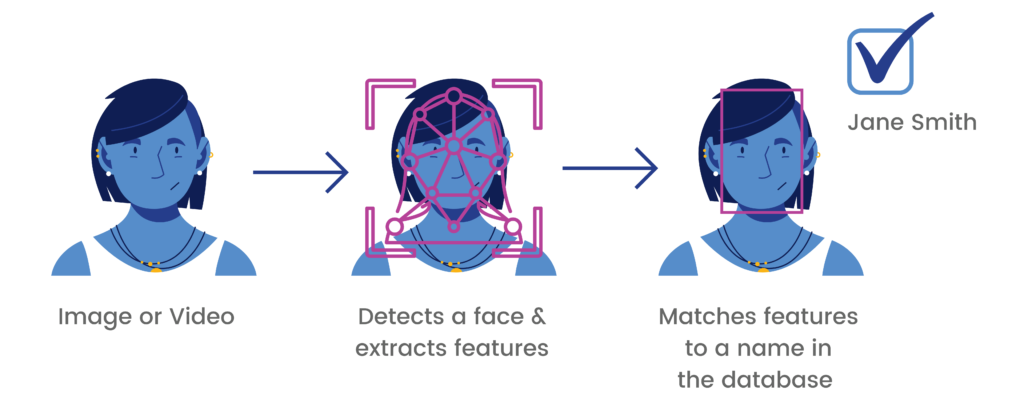
\includegraphics[width=\textwidth]{images/presentation/face_recognition.png}
            \caption{Face Recognition problem}
        \end{figure}
	\end{frame}

     \begin{frame}{ML in Information Security: Cancelable Biometrics}
    	    \begin{figure}
            \centering
                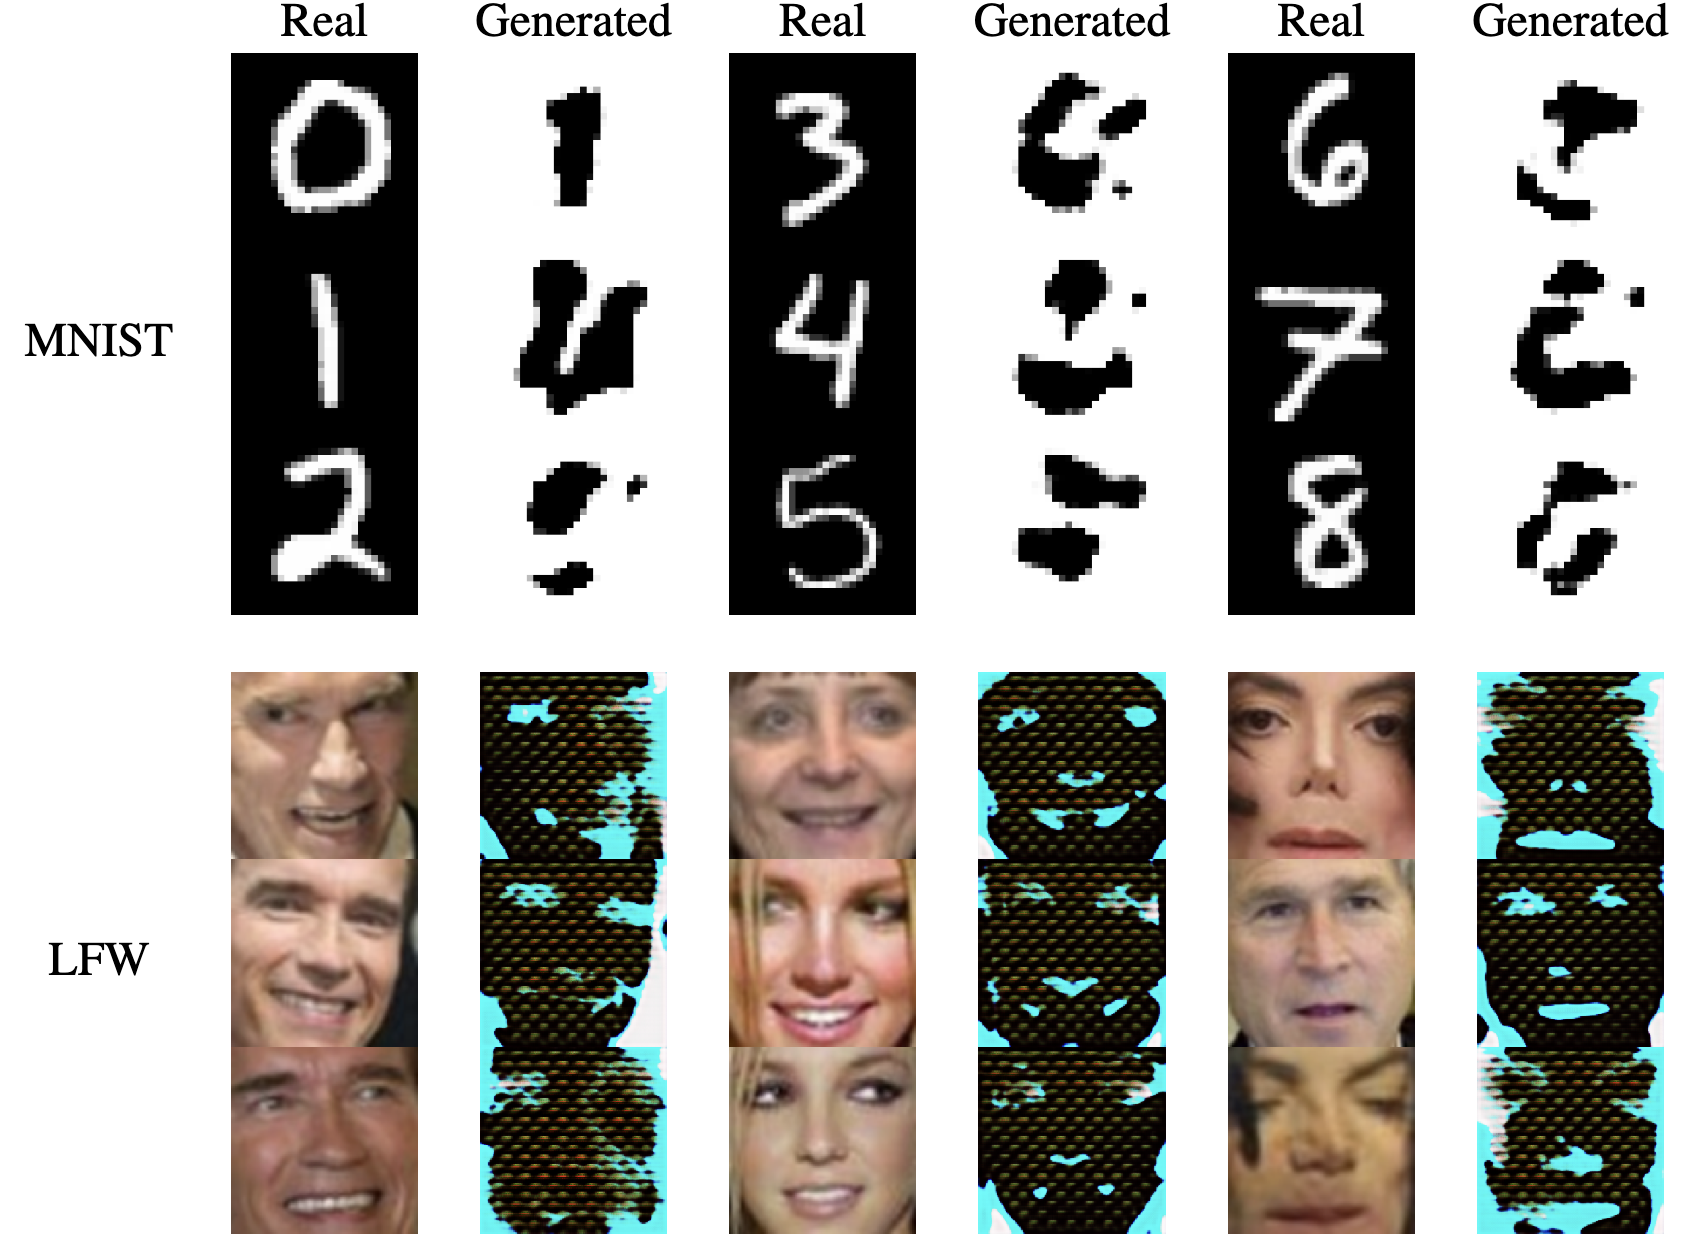
\includegraphics[width=0.7\textwidth]{images/presentation/cancelable.png}
                \caption{Cancelable Biometrics. Real and generated images are identifiable by the neural network}
            \end{figure}
    	\end{frame}

    \begin{frame}{ML is fun! Pix2Pix}
	    \begin{figure}
        \centering
            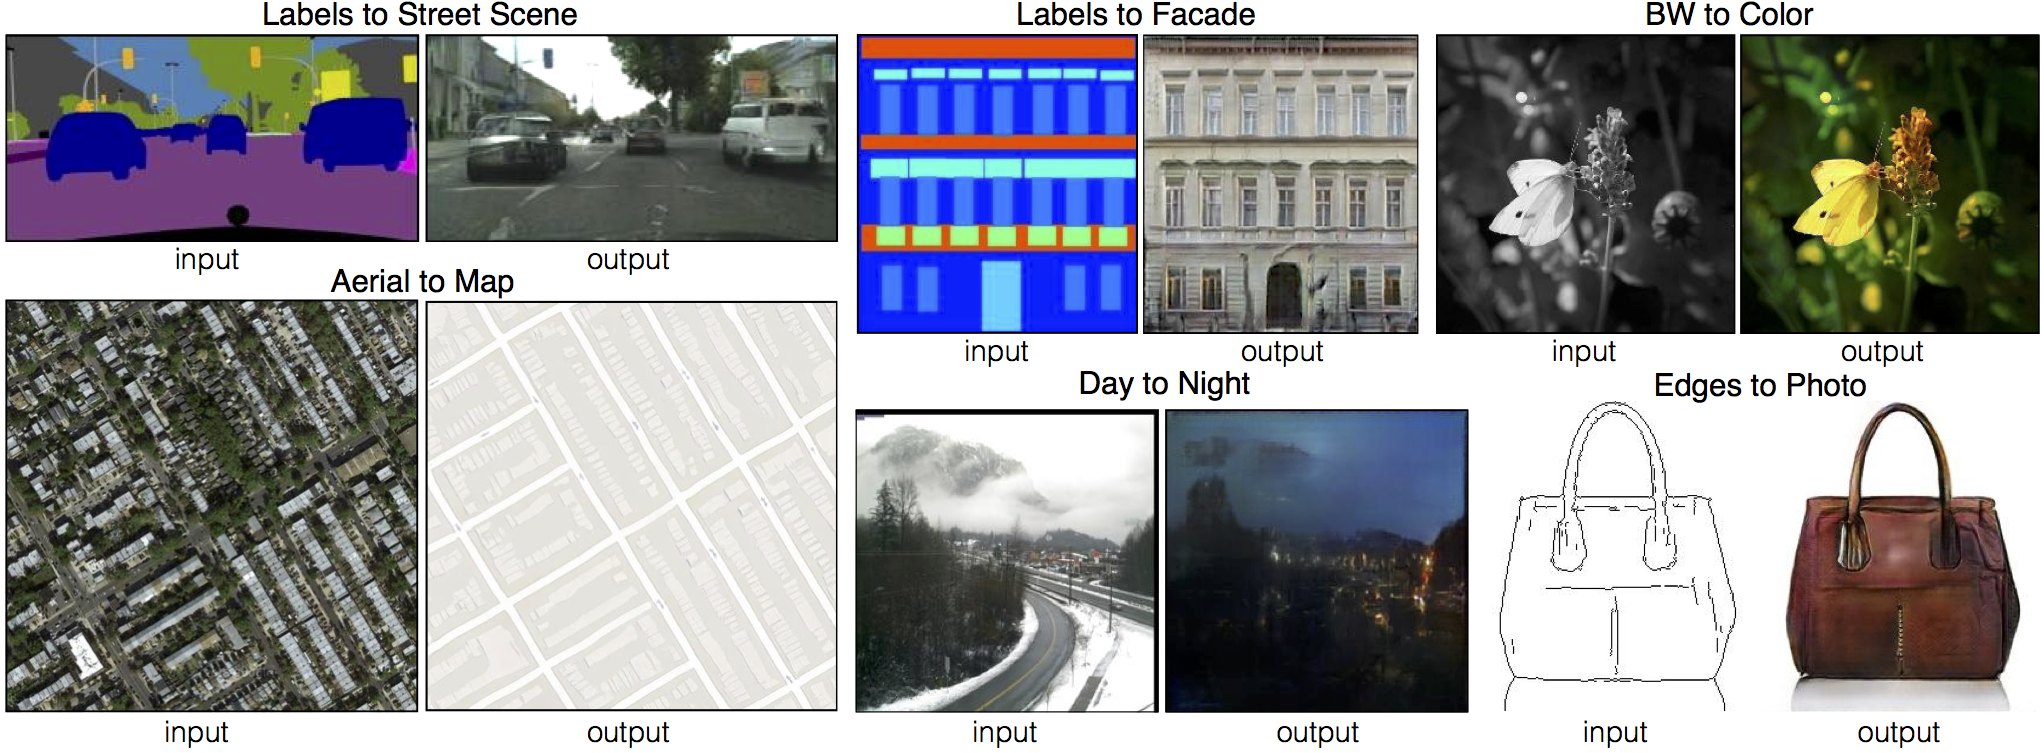
\includegraphics[width=\textwidth]{images/presentation/pix2pix.png}
            \caption{Image-to-image translation. \textit{Pix2Pix}. See this url for reference: \href{https://phillipi.github.io/pix2pix/}{phillipi.github.io/pix2pix/}}
        \end{figure}
	\end{frame}

     \begin{frame}{ML is fun! Neural Transfer}
	    \begin{figure}
        \centering
            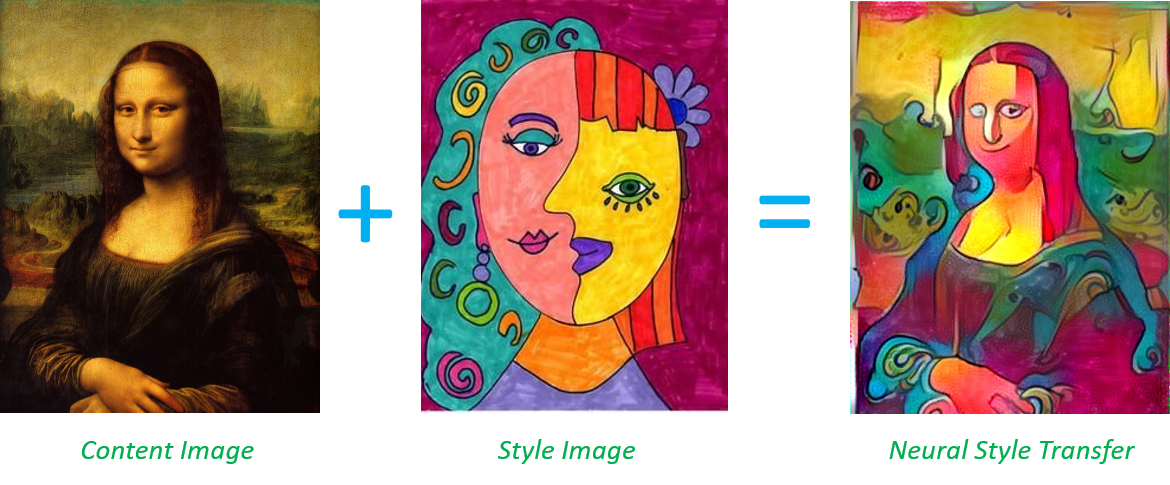
\includegraphics[width=\textwidth]{images/presentation/neural-transfer.png}
            \caption{Neural transfer. See this link if you want to learn more: \href{https://www.v7labs.com/blog/neural-style-transfer}{https://www.v7labs.com/blog/neural-style-transfer}.}
        \end{figure}
	\end{frame}

     \begin{frame}{ML is fun! ChatGPT}
	    \begin{figure}
        \centering
            
\includegraphics[width=\textwidth]{images/presentation/chatgpt.jpg}
            \caption{Do I actually need to explain what it is?}
        \end{figure}
	\end{frame}
    \subsection{Definitions}
	\begin{frame}{AI vs ML vs DL}
	    \begin{figure}
        \centering
            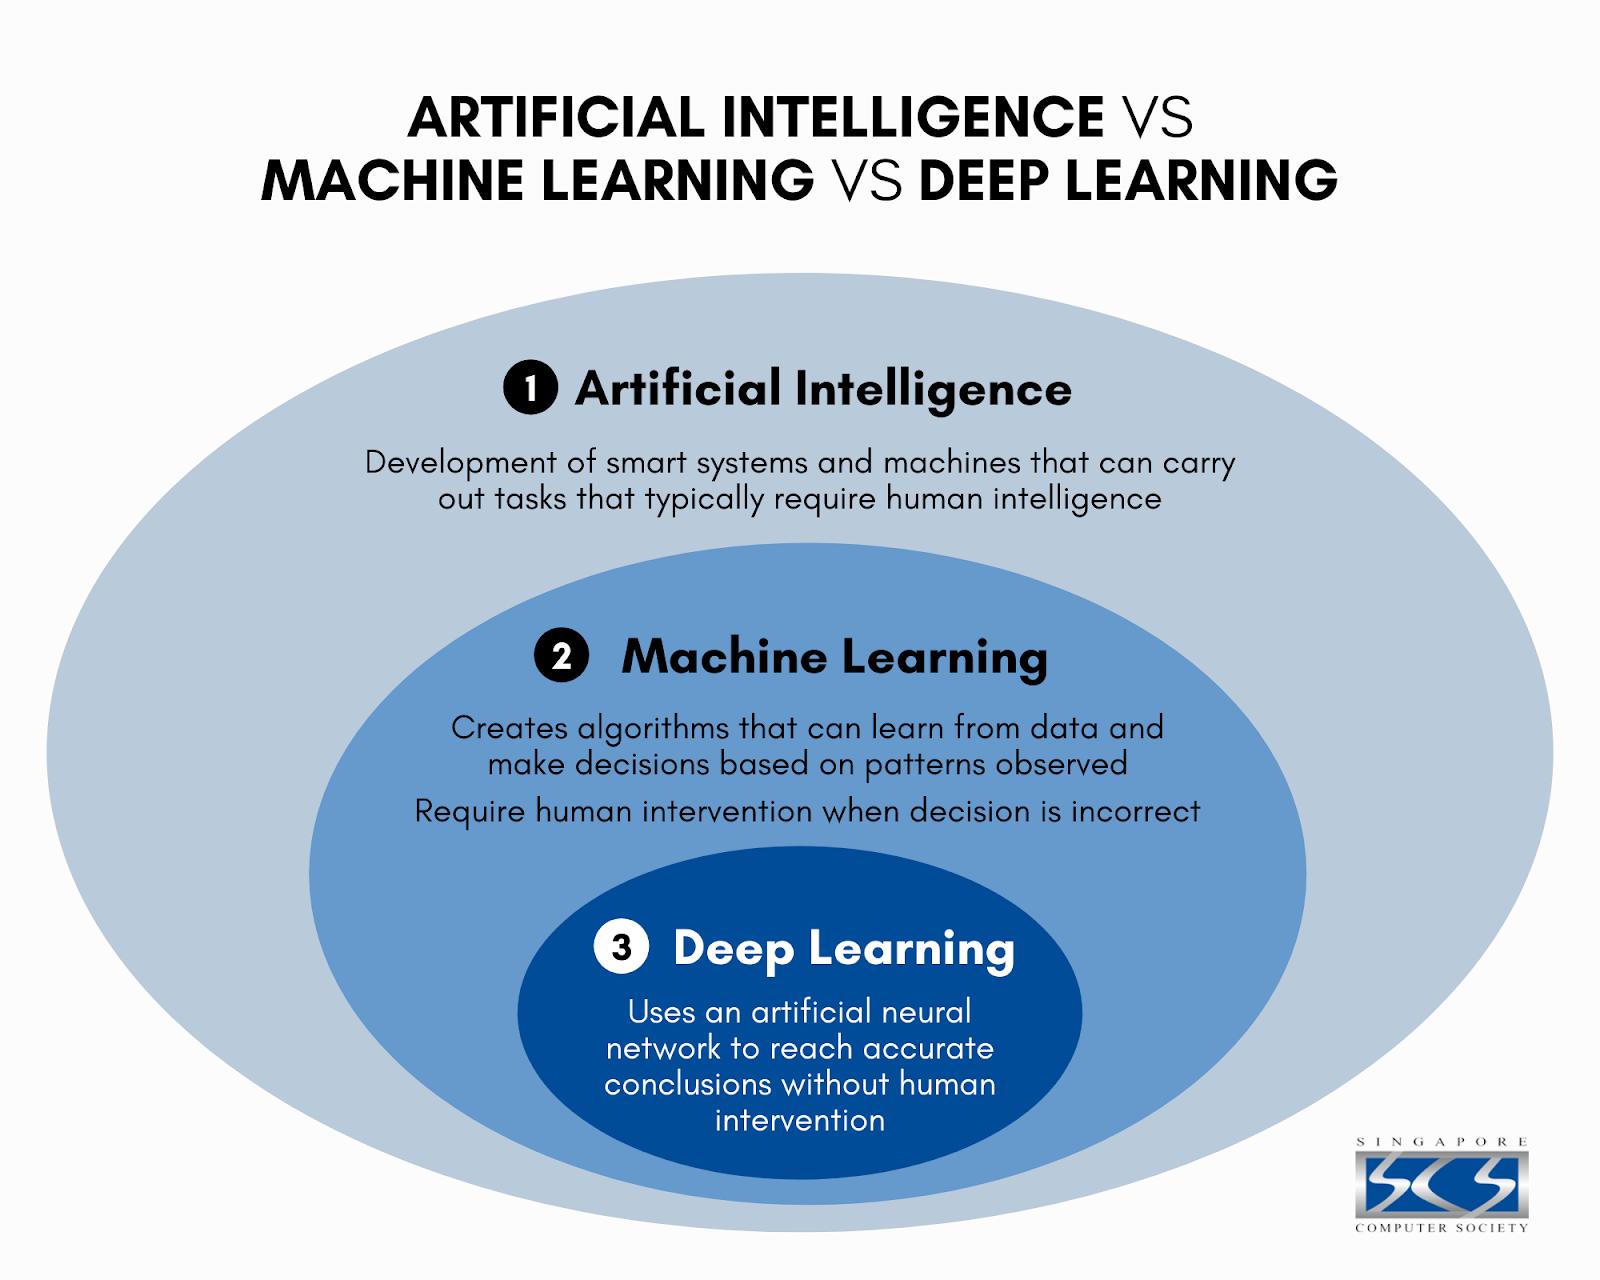
\includegraphics[width=0.8\textwidth]{images/presentation/mlvsdl.png}
        \end{figure}
	\end{frame}
    \begin{frame}{What is Machine Learning?}
        \begin{block}{Informal definition}
        \textbf{Machine Learning} is a field of study that learns to build a certain \textbf{function} $f$, based on the given data $\mathcal{D}$, that can give useful information about new upcoming data $\mathcal{D}_{\text{new}}$ following the same distribution as $\mathcal{D}$. 
        \end{block}

        \begin{figure}
        \centering
            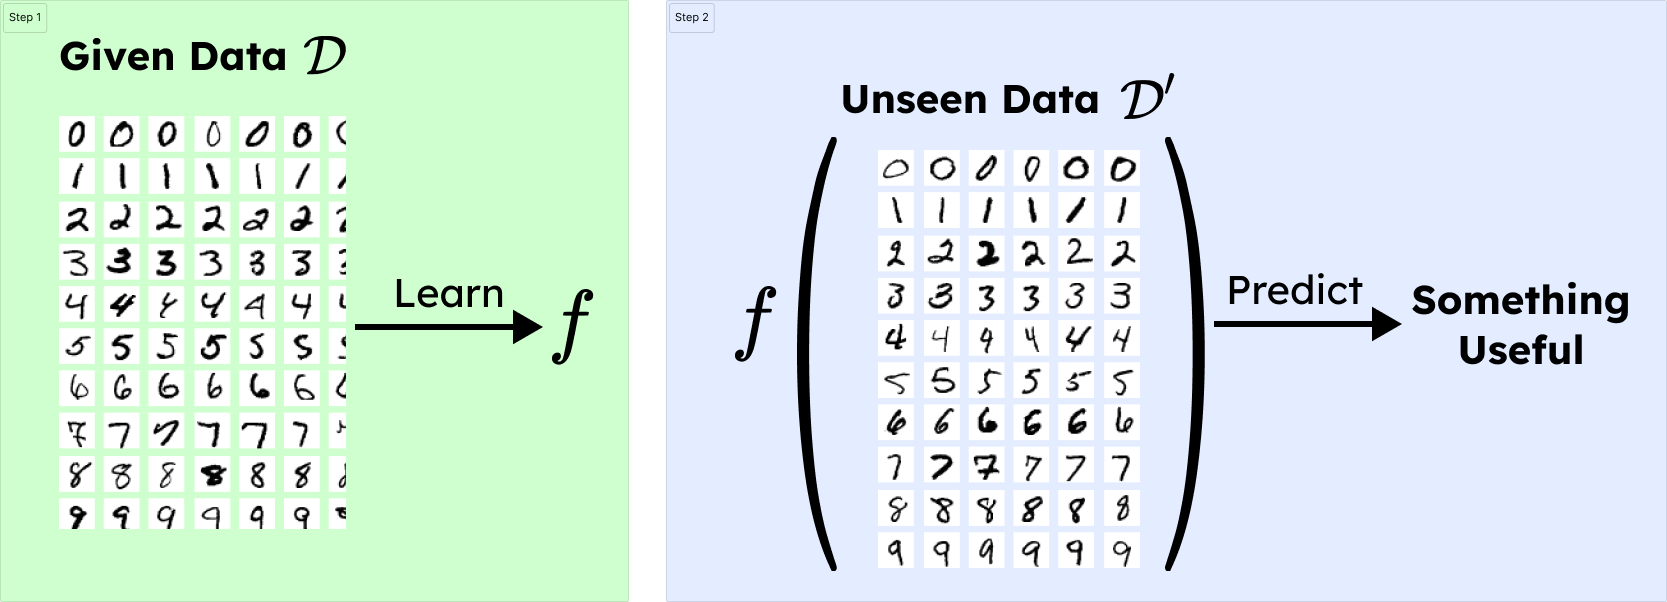
\includegraphics[width=\textwidth]{images/presentation/def.png}
        \end{figure}
    \end{frame}
	
    \begin{frame}{A few words about math}
        Does ML involve a lot of math? \textbf{Yes}.

        Do you necessarily need to know \textit{advanced} math to do ML? \textbf{No}.

        Do you need \textit{basic} understand of math to do ML? \textbf{Yes}.

        \begin{figure}
        \centering
            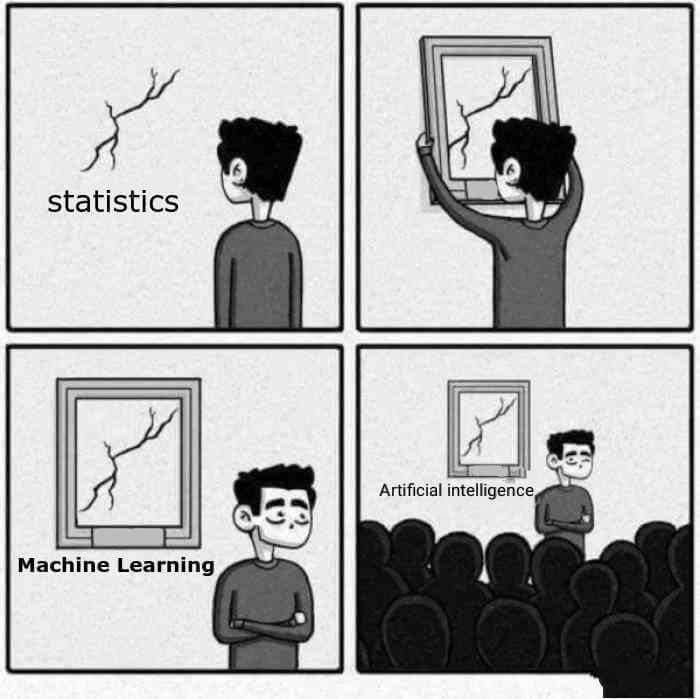
\includegraphics[width=0.5\textwidth]{images/presentation/meme.jpg}
        \end{figure}
    \end{frame}
    \begin{frame}{Math in Papers: Good Example}
        Papers \textbf{love} formality, but the core is intuitive and quite often straightforward.

        \begin{figure}
        \centering
            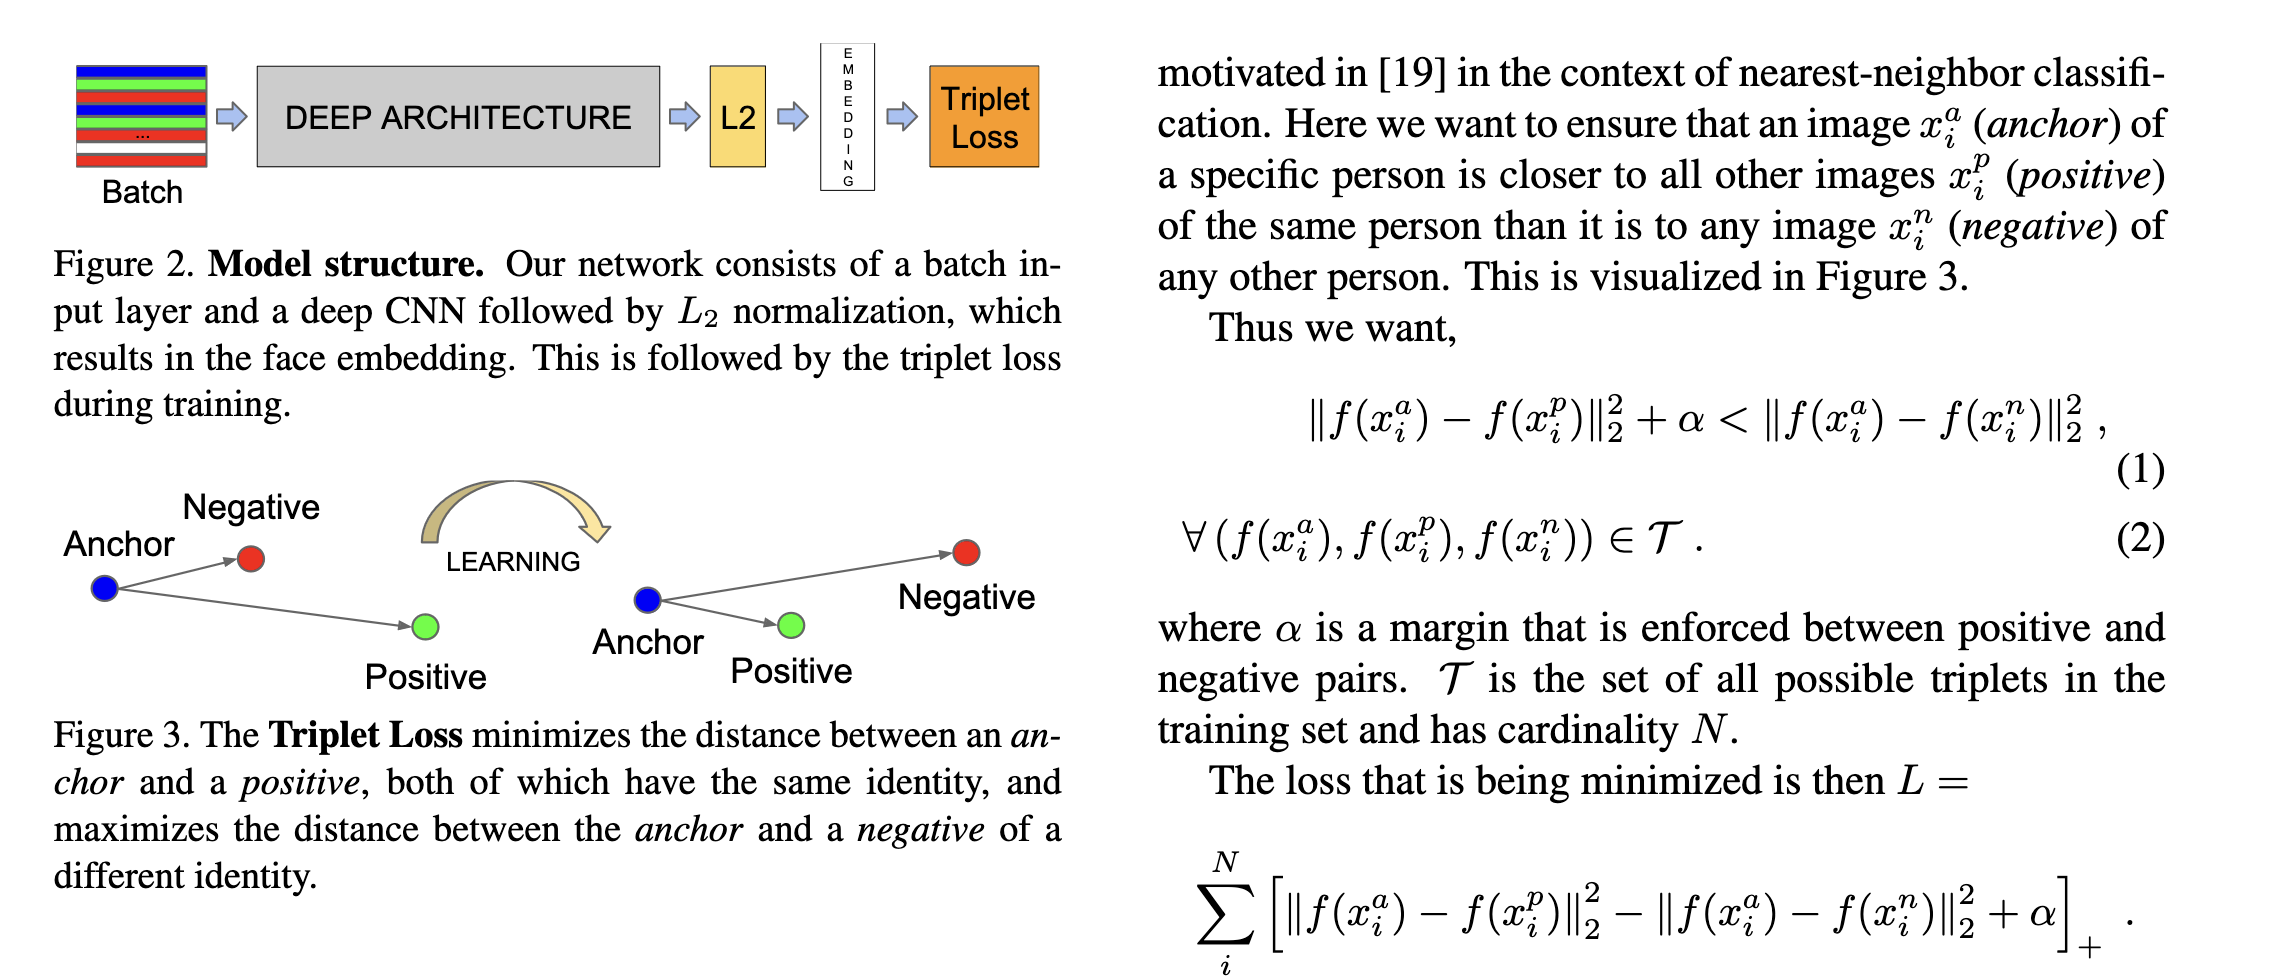
\includegraphics[width=\textwidth]{images/presentation/facenet.png}
            \caption{\textit{FaceNet} paper. See \href{https://arxiv.org/pdf/1503.03832.pdf}{here} for reference.}
        \end{figure}
    \end{frame}
    
    \subsection{Paradigms}
	\begin{frame}{Supervised Learning}
		\begin{columns}
        \begin{column}{0.5\textwidth}
	    \begin{block}{Supervised Learning}
        Given a pair of inputs and desired outputs (labels) 
         \[
         (x_1,y_1),(x_2,y_2),\dots,(x_n,y_n),
         \]
         build a function $f$ that can effectively map inputs to outputs.
	    \end{block}
        
        \begin{exampleblock}{Example}
        Given a set of labeled images of dogs and cats, build an NN that predicts whether an image belongs to a cat or a dog.
        \end{exampleblock}
        \end{column}
        \begin{column}{0.5\textwidth}
        \begin{figure}
        \centering
            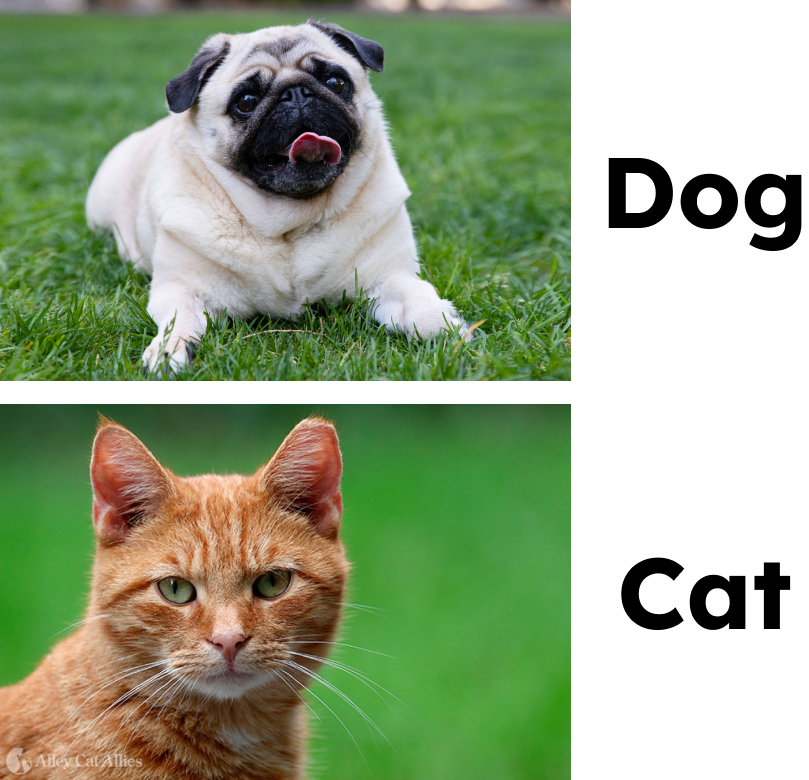
\includegraphics[width=\textwidth]{images/presentation/classification.png}
            \caption{Supervised learning example}
        \end{figure}
        \end{column}
        \end{columns}
	\end{frame}

    \begin{frame}{Unsupervised Learning}
        \begin{columns}
        % Description
        \begin{column}{0.5\textwidth}
        \begin{block}{Supervised Learning}
        Given a dataset with unlabeled data $x_1,x_2,\dots,x_n$, explore patterns in data.
	    \end{block}

        \begin{exampleblock}{Example}
        Document analysis -- given a vast library of different research papers, put them into groups according to the selected group of criteria. 
        \end{exampleblock}
        \end{column}
        \begin{column}{0.5\textwidth}
            
        \begin{figure}
        \centering
            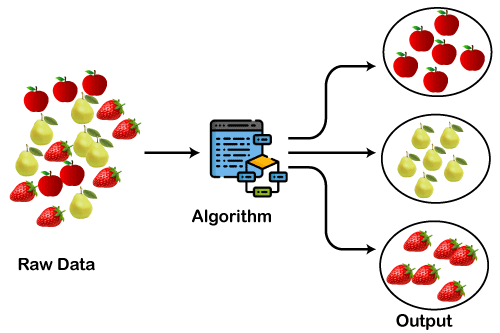
\includegraphics[width=\textwidth]{images/presentation/clustering.png}
            \caption{Clustering task}
        \end{figure}

        \end{column}
        \end{columns}
	\end{frame}

    \begin{frame}{Reinforcement Learning}
        \begin{columns}
        % Description
        \begin{column}{0.5\textwidth}
        \begin{block}{Supervised Learning}
        Producing actions $a_1,a_2,\dots,a_n$ which affect the environment, and receiving rewards $r_1,\dots,r_m$ learn to act such that it maximizes the reward. 
	    \end{block}

        \begin{exampleblock}{Example}
        Writing a bot that can complete levels in a videogame.
        \end{exampleblock}
        \end{column}
        \begin{column}{0.5\textwidth}
            
        \begin{figure}
        \centering
            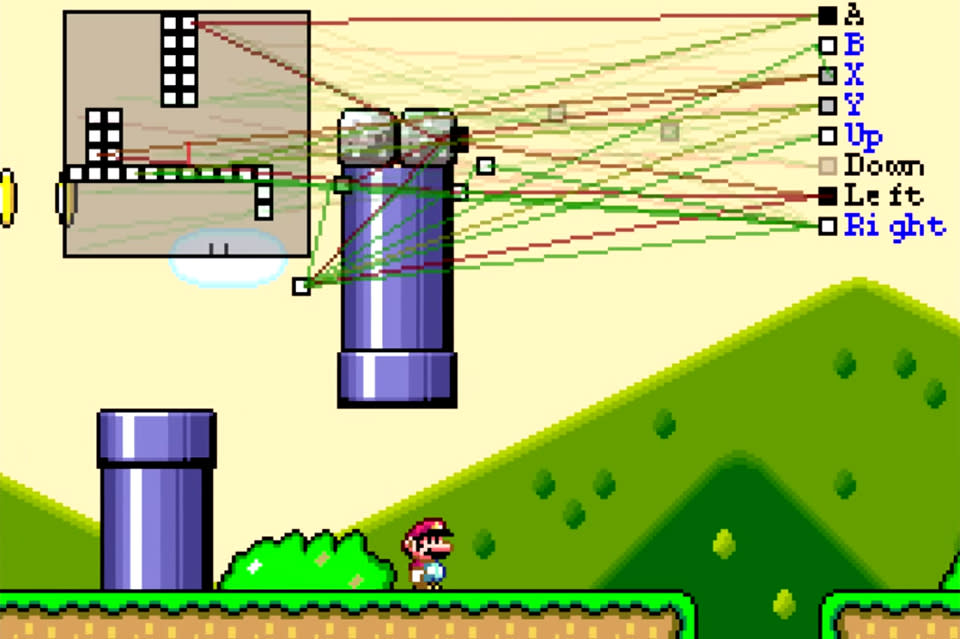
\includegraphics[width=\textwidth]{images/presentation/mario.jpg}
            \caption{Reinforcement Learning example}
        \end{figure}

        \end{column}
        \end{columns}
    \end{frame}

    \begin{frame}{A bit of interactivity: object detection}
        \begin{exampleblock}{Question \#1}
            Given a set of images with people, dogs, and cars marked, build a model that detects these objects on the photo. Is that a supervised, unsupervised, or reinforcement task? Why?
        \end{exampleblock}

        \begin{figure}
        \centering
            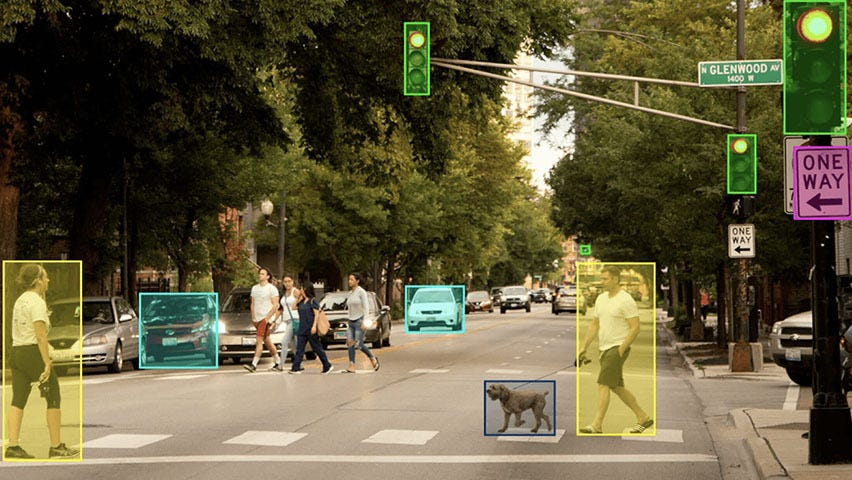
\includegraphics[width=0.6\textwidth]{images/presentation/bounding_boxes.jpg}
            \caption{Illustration for question 1}
        \end{figure}
    \end{frame}

    \begin{frame}{A bit of interactivity: your own examples}
        \begin{exampleblock}{Question \#2}
            Give your own examples of (a) -- supervised learning, (b) -- unsupervised learning, and (c) -- reinforcement learning.
        \end{exampleblock}

        \begin{figure}
        \centering
            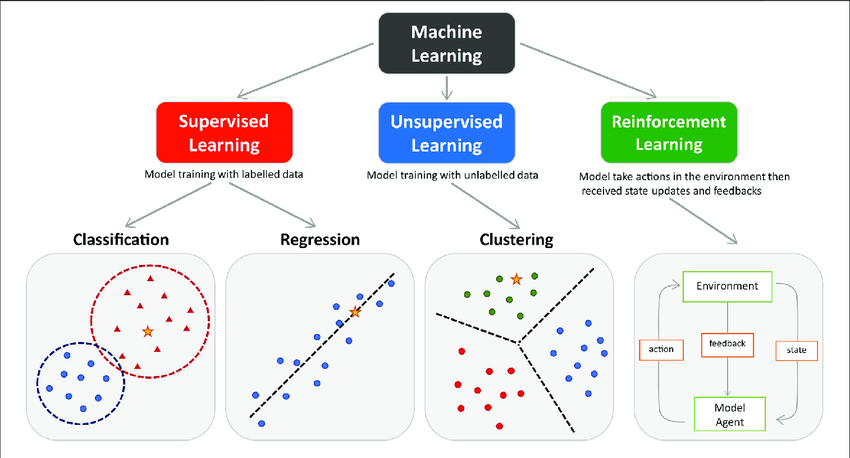
\includegraphics[width=0.8\textwidth]{images/presentation/types_of_ml.png}
        \end{figure}
    \end{frame}

    \section{Building the first Neural Network!}

    \subsection{Problem statement}
    
    \begin{frame}
        \frametitle{Problem Statement}

        \begin{block}{``Hello World'' in Machine Learning}
            Write a program that, based on the $28 \times 28$ grayscale image of a digit, predicts what digit it is. You are given a set of images $\{x_i\}_{i=1}^n$ and corresponding labels $\{y_i\}_{i=1}^n, \, y_i \in \{0,\dots,9\}$.
        \end{block}
        
        \begin{figure}
        \centering
            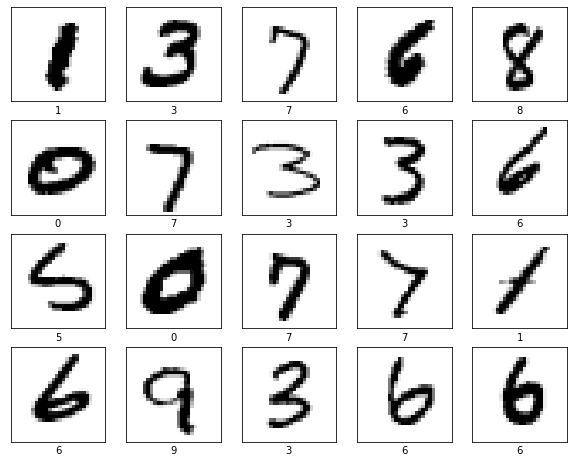
\includegraphics[width=0.4\textwidth]{images/presentation/mnist_2.png}
            \caption{MNIST dataset}
        \end{figure}
    \end{frame}

    \begin{frame}
        \frametitle{Neural Network}

        To define what \textbf{\textcolor{green}{Neural} \textcolor{blue}{Network}} is, we need to define:
        \begin{enumerate}
            \item What is a \textcolor{green}{\textbf{neuron}}?
            \item How \textcolor{green}{\textbf{neurons}} form a \textbf{\textcolor{blue}{network}}?
        \end{enumerate}

        The first is simple! 

        \begin{definition}
            \textbf{Neuron} is a number. Really. That's just it...

            A bit more formally, this is a node in the network, possessing an \textbf{activation}, which is just a number indicating how active is the neuron.
        \end{definition}
    \end{frame}

    \begin{frame}{Neurons in the context of an image}
        \begin{figure}
        \centering
            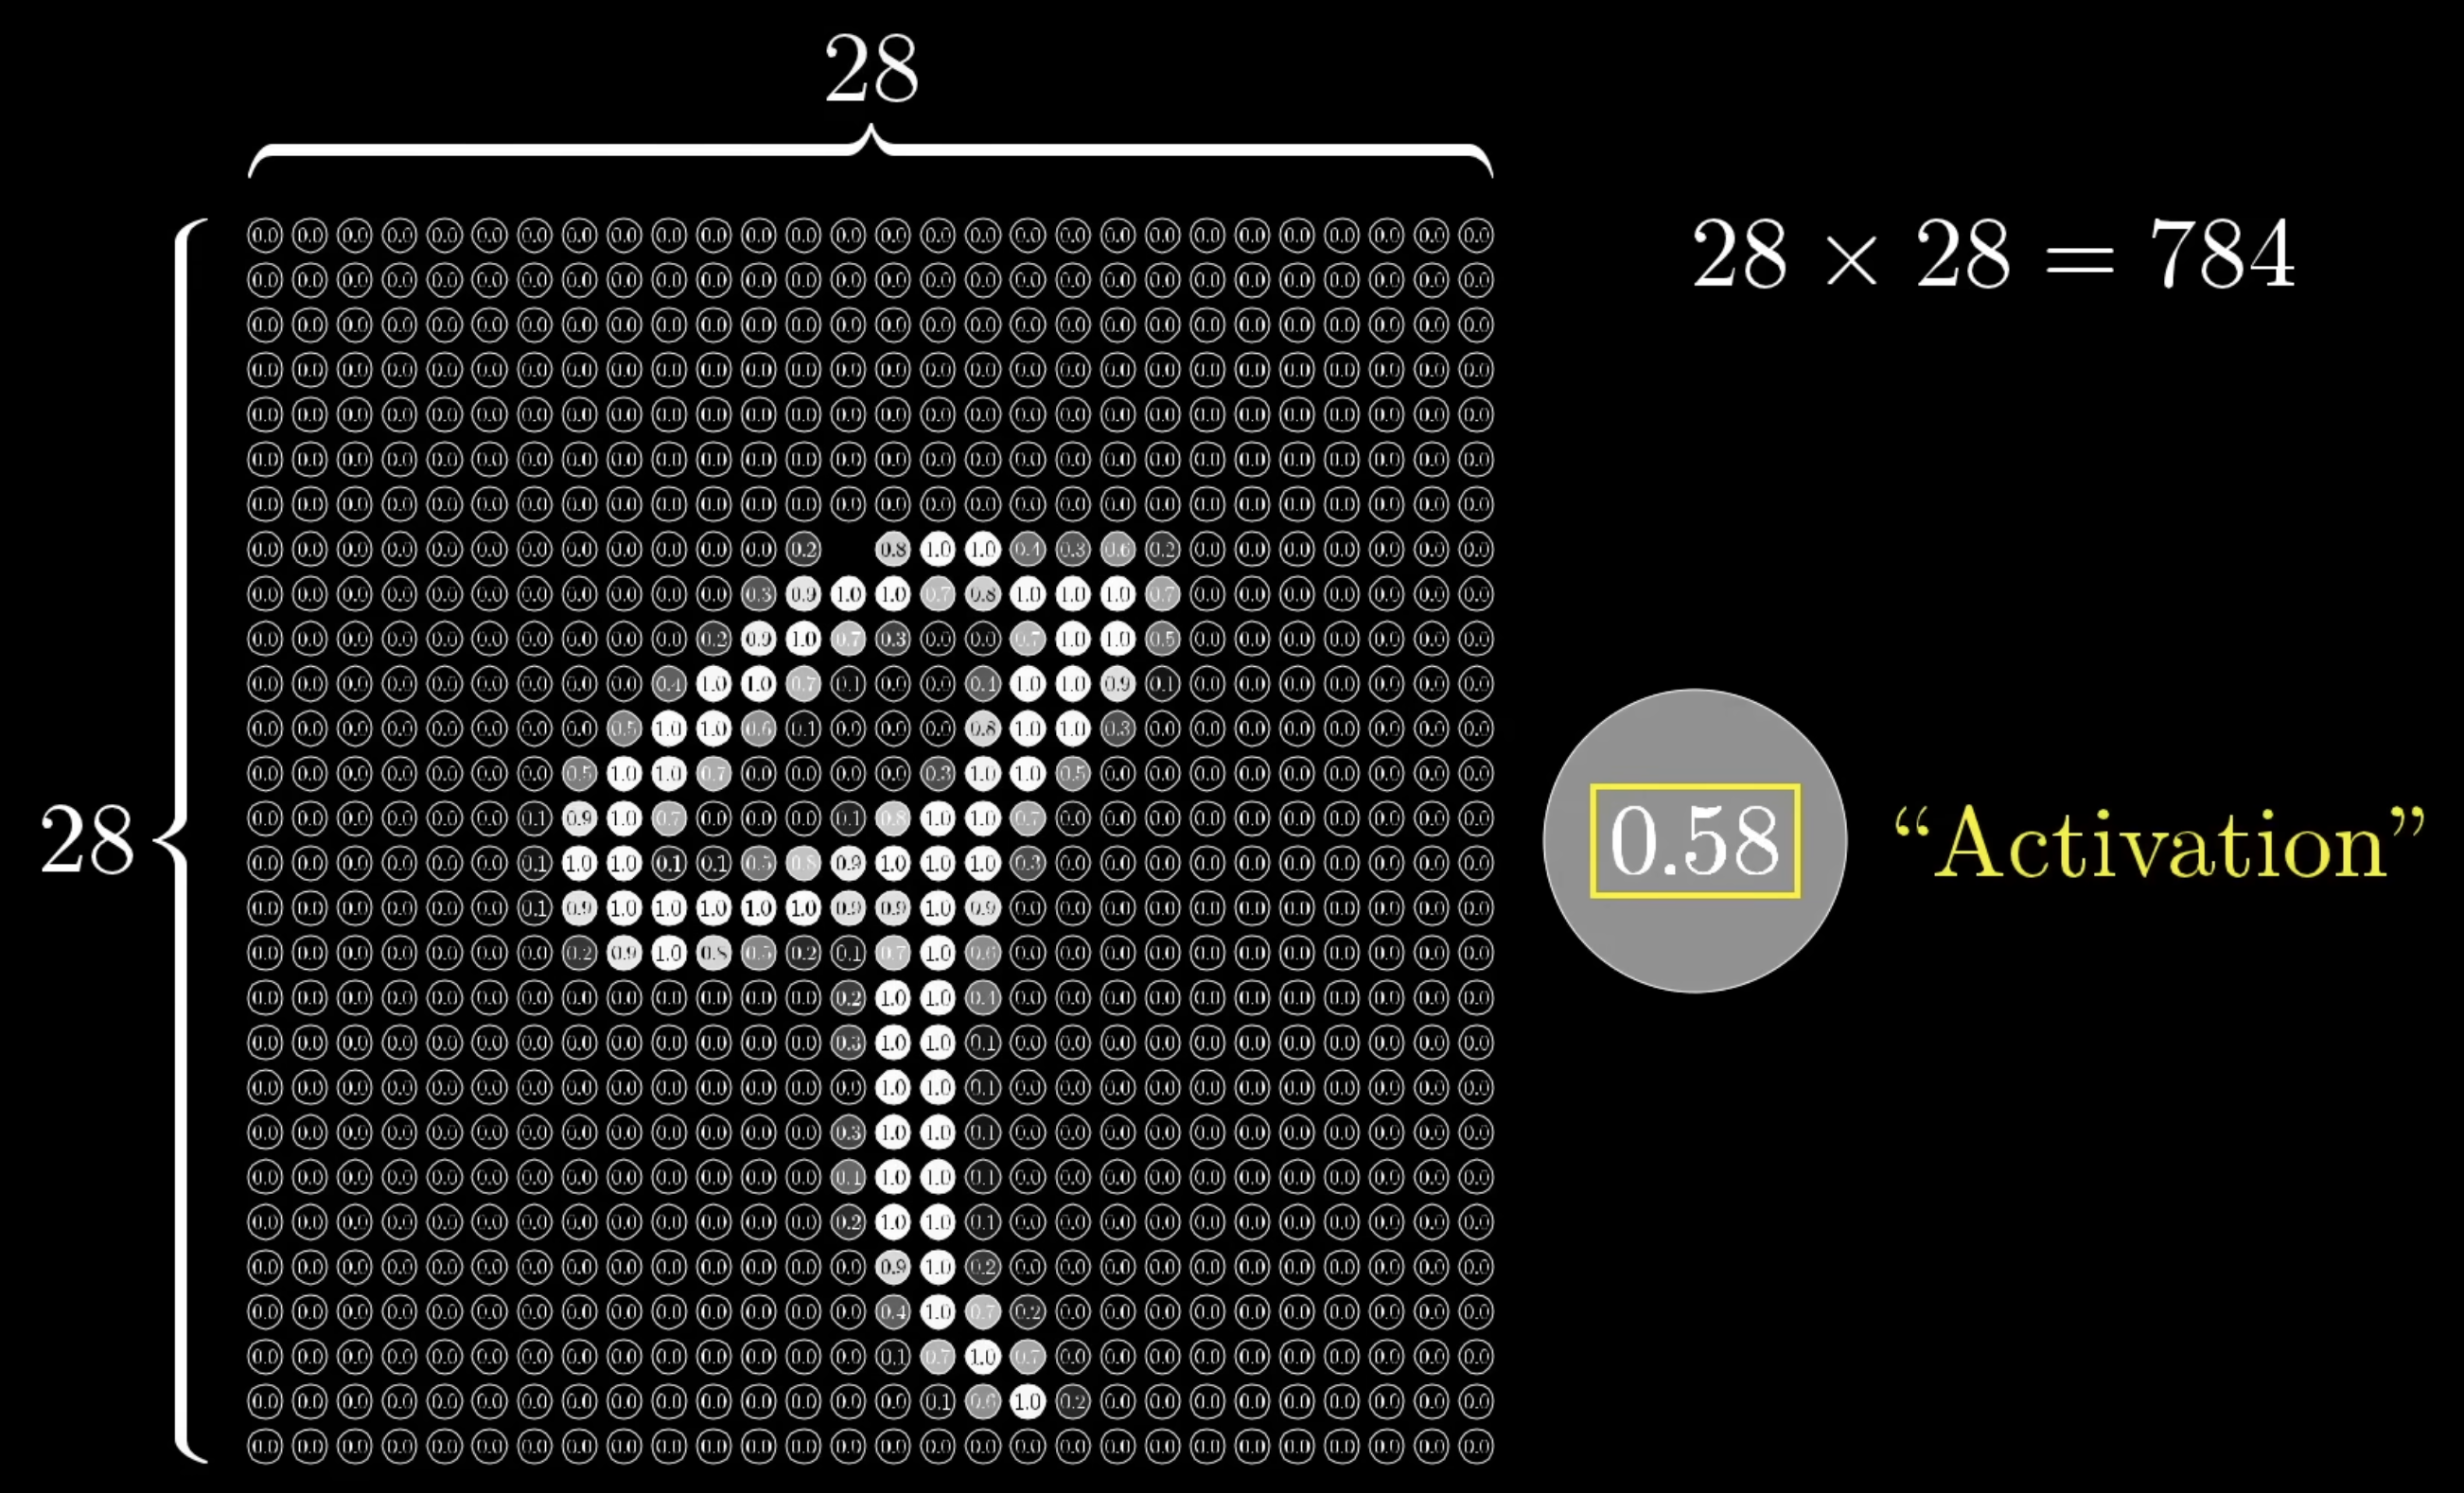
\includegraphics[width=0.8\textwidth]{images/presentation/image_activations.png}
            \caption{Each pixel of an image is an individual neuron, having an activation between $0$ and $1$. Image taken from \href{https://www.youtube.com/watch?v=aircAruvnKk&list=PLZHQObOWTQDNU6R1_67000Dx_ZCJB-3pi}{3Blue1Brown video}.}
        \end{figure}
    \end{frame}

    \begin{frame}{Flattening...}
        \begin{figure}
        \centering
            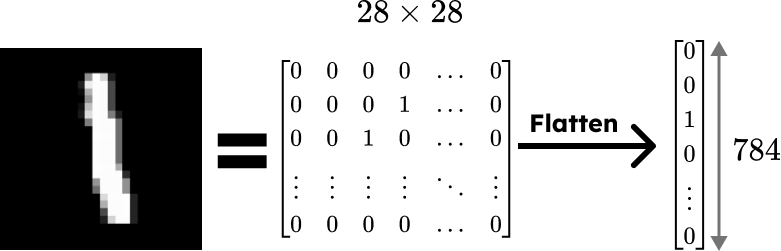
\includegraphics[width=\textwidth]{images/presentation/flatten.png}
            \caption{Forming a single vector from the image}
        \end{figure}
    \end{frame}

    \subsection{Forward propagation}
    \begin{frame}{Neural Network Layer}
        Denote $i^{\text{th}}$ activation (the neuron's value) in the $\ell^{\text{th}}$ layer as $a^{\langle \ell\rangle}_i$. Let us define activation of $a^{\langle 2\rangle}_1$ in terms of first-layer activations $a^{\langle 1 \rangle}_i, \; i = 1,2,\dots,784$. 
    
        \begin{figure}
        \centering
            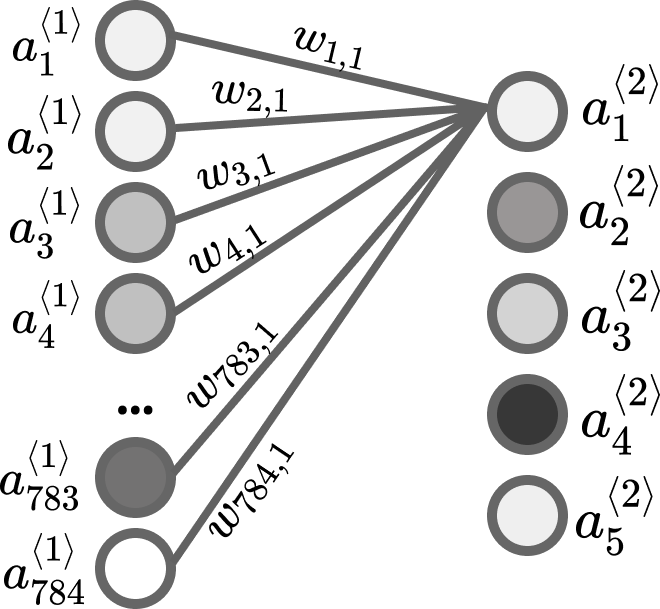
\includegraphics[width=0.4\textwidth]{images/presentation/layer.png}
            \caption{First hidden layer in our network}
        \end{figure}
    \end{frame}

    \begin{frame}{Contribution from the first layer}
        Suppose that ``importance'' (formally, a weight) of the first neuron in the first layer contributing to the first neuron in the second layer is $w_{1,1}$. Then, $a_1^{\langle 1 \rangle}$ contribution to the value of $a_1^{\langle 2\rangle}$ is $w_{1,1}a_1^{\langle 1 \rangle}$. 
    
        \begin{figure}
        \centering
            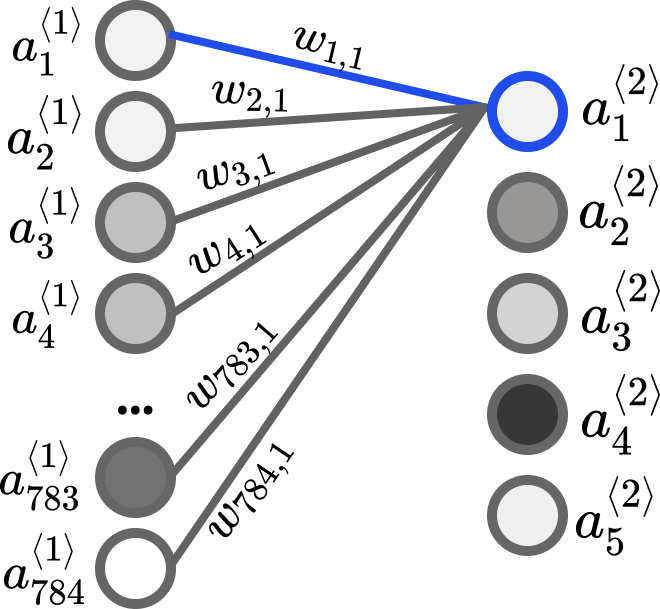
\includegraphics[width=0.4\textwidth]{images/presentation/layer_first_selected.png}
            \caption{First hidden layer in our network}
        \end{figure}
    \end{frame}

    \begin{frame}{Total contribution}
        Similarly, second neuron of the first layer has a contribution of $w_{2,1}a_2^{\langle 1 \rangle}$ to the first neuron in the second layer. Similarly, the sum of all contributions is:
        \[
        a_1^{\langle 2 \rangle} = w_{1,1}a_1^{\langle 1 \rangle} + w_{2,1}a_2^{\langle 1 \rangle} + \dots + w_{784,1}a_{784}^{\langle 1 \rangle} = \sum_{i=1}^{784}w_{i,1}a_i^{\langle 1 \rangle}
        \]
    
        \begin{figure}
        \centering
            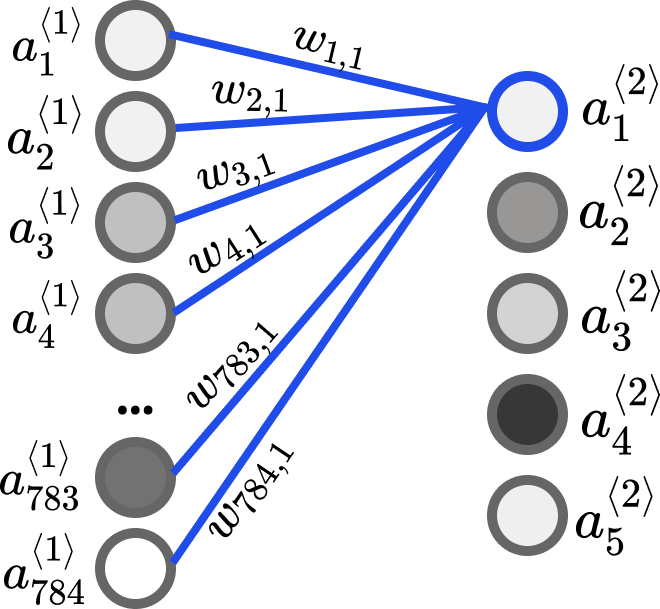
\includegraphics[width=0.4\textwidth]{images/presentation/layer_all_selected.png}
        \end{figure}
    \end{frame}

    \begin{frame}{A bit of interactivity}
    \begin{columns}
        \begin{column}{0.5\textwidth}
            \begin{exampleblock}{Question \#1}
                What value of $a_1^{\langle 2 \rangle}$ we would get if all $w_{i,1}$ were $0$?
            \end{exampleblock}
            \begin{exampleblock}{Question \#2}
                What value of $a_1^{\langle 2 \rangle}$ we would get if all $w_{i,1}$ were $0$ except for $w_{j,1}=1$?
            \end{exampleblock}
            \begin{exampleblock}{Question \#3}
                What if all $w_{i,1}=1$?
            \end{exampleblock}
        \end{column}
        \begin{column}{0.5\textwidth}
            \begin{figure}
            \centering
                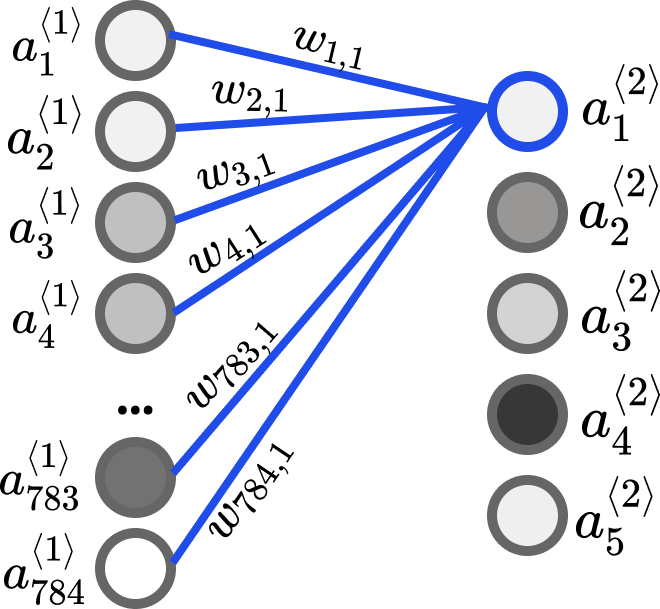
\includegraphics[width=\textwidth]{images/presentation/layer_all_selected.png}
            \end{figure}
        \end{column}
    \end{columns}
    \end{frame}

    \begin{frame}{Summing for every activation}
        \begin{columns}
        \begin{column}{0.7\textwidth}
        And now we have \textbf{TONS} of connections:
        \begin{gather*}
            a_1^{\langle 2 \rangle} = w_{1,1}a_1^{\langle 1 \rangle} + w_{2,1}a_2^{\langle 1 \rangle} + \dots + w_{784,1}a_{784}^{\langle 1 \rangle} \\
            a_2^{\langle 2 \rangle} = w_{2,1}a_1^{\langle 1 \rangle} + w_{2,2}a_2^{\langle 1 \rangle} + \dots + w_{784,2}a_{784}^{\langle 1 \rangle} \\
            \vdots \\
            a_5^{\langle 2 \rangle} = w_{1,5}a_1^{\langle 1 \rangle} + w_{2,5}a_2^{\langle 1 \rangle} + \dots + w_{784,5}a_{784}^{\langle 1 \rangle}
        \end{gather*}

        \begin{block}{Question}
            How can we write this expression concisely?

            \textbf{Hint:} Maybe vector and matrix notation could help?
        \end{block}
        
        \end{column}

        \begin{column}{0.3\textwidth}
        \begin{figure}
        \centering
            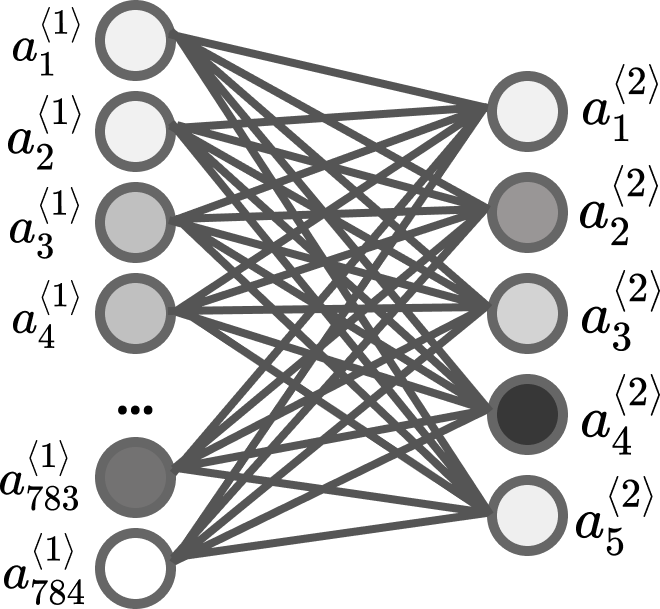
\includegraphics[width=\textwidth]{images/presentation/layer_all_all.png}
        \end{figure}
        \end{column}
        \end{columns}
    \end{frame}

    \begin{frame}{A bit of Linear Algebra}
        \begin{columns}
        \begin{column}{0.7\textwidth}
        Answer:
        \[
        \begin{bmatrix}
            a_1^{\langle 2 \rangle} \\
            \vdots \\
            a_5^{\langle 2 \rangle}
        \end{bmatrix} = \begin{bmatrix}
            w_{1,1} & \dots & w_{784,1} \\
            \vdots & \ddots & \vdots \\
            w_{1,5} & \dots & w_{784,5}
        \end{bmatrix}\begin{bmatrix}
            a_1^{\langle 1\rangle} \\
            \vdots \\
            a_{784}^{\langle 1\rangle}
        \end{bmatrix}
        \]

        Or even more concisely!
        \[
        \mathbf{a}^{\langle \ell + 1\rangle} = \mathbf{W}^{\langle \ell\rangle}\mathbf{a}^{\langle \ell \rangle}
        \]

        However, in this case, elements of $\mathbf{a}^{\langle \ell + 1\rangle}$ can take any values on the real line, but we want values in range $(0,1)$. What to we do?
        \end{column}

        \begin{column}{0.3\textwidth}
        \begin{figure}
        \centering
            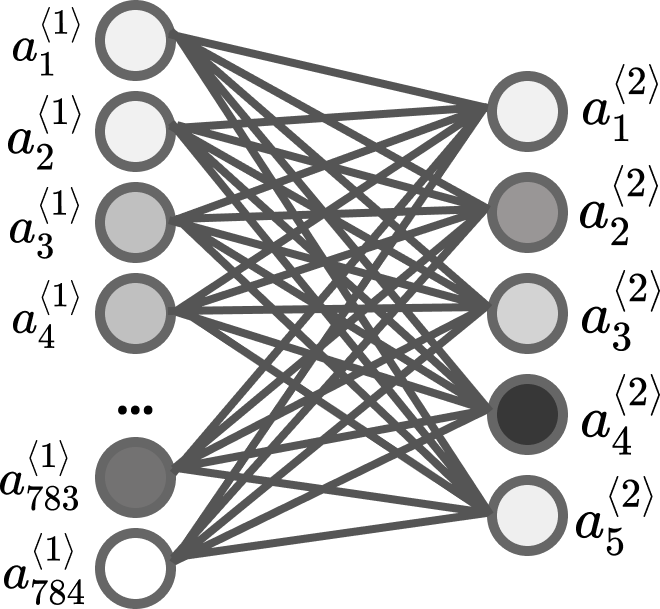
\includegraphics[width=\textwidth]{images/presentation/layer_all_all.png}
        \end{figure}
        \end{column}
        \end{columns}
    \end{frame}

    \begin{frame}{Activation function}
        Let us apply sigmoid function $\sigma(x)$ to all retrieved values! It will map any value to the interval $(0,1)$.
        \begin{figure}
        \centering
            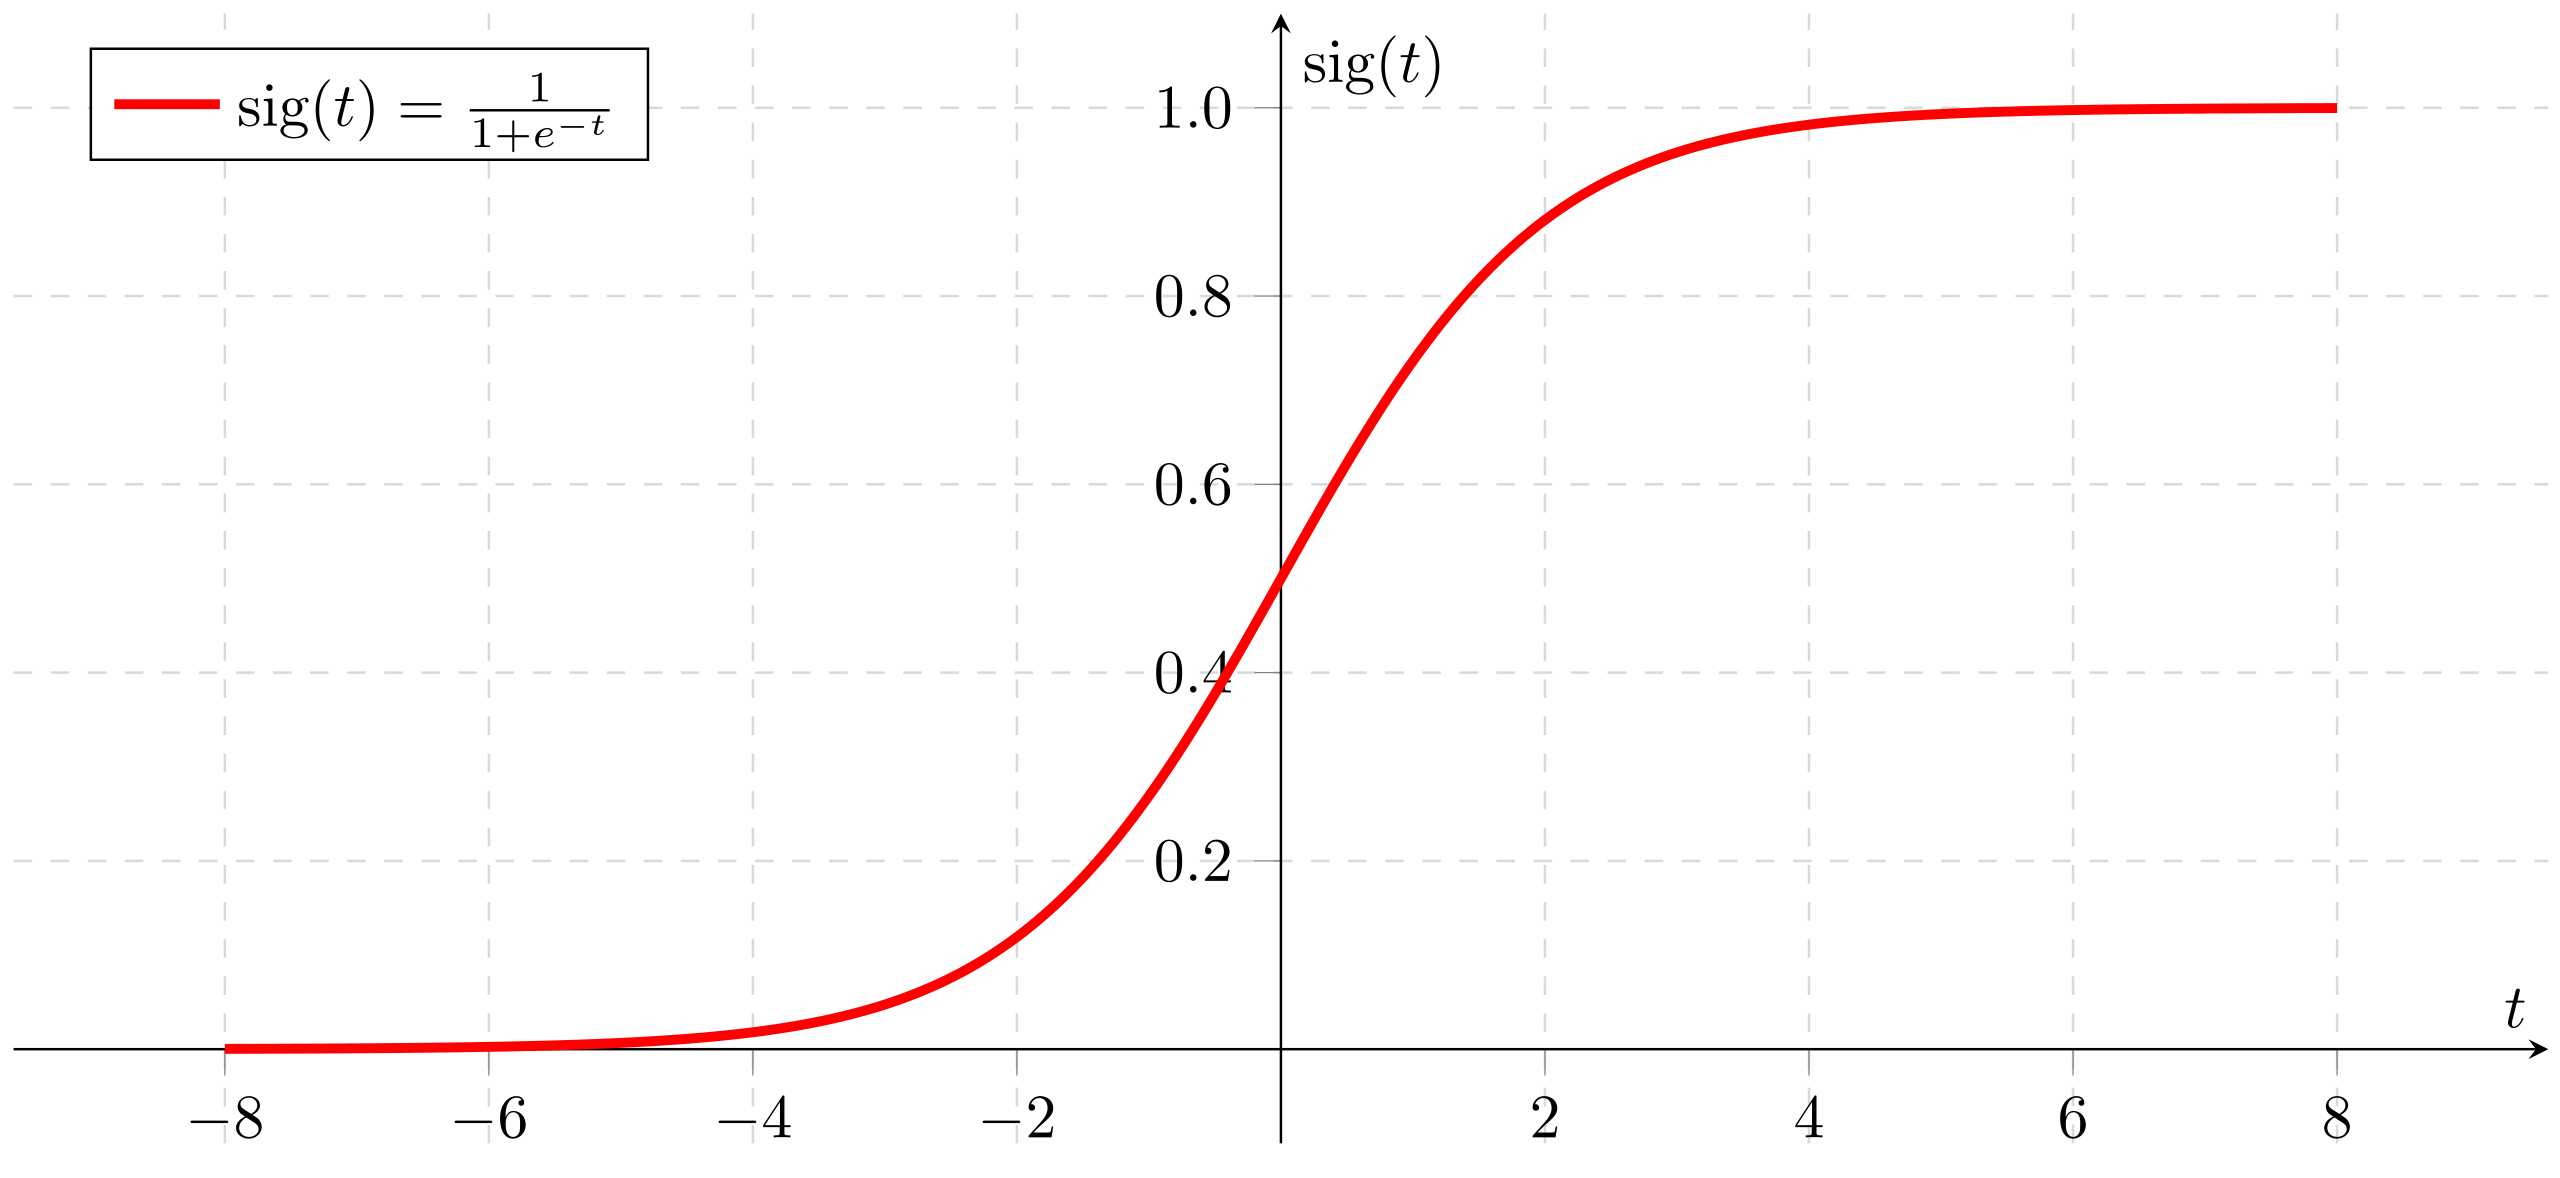
\includegraphics[width=\textwidth]{images/presentation/sigmoid.png}
        \end{figure}
    \end{frame}

    \begin{frame}{Neural Network Layer}
        \begin{columns}
        \begin{column}{0.7\textwidth}
        Thus, let us do
        \[
        \mathbf{a}^{\langle\ell+1\rangle} = \sigma\left(\mathbf{W}^{\langle \ell\rangle}\mathbf{a}^{\langle\ell\rangle}\right)
        \]
        To make neural network a bit more complicated, let's add an ``offset'':
        \[
        \mathbf{a}^{\langle\ell+1\rangle} = \sigma\left(\mathbf{W}^{\langle \ell\rangle}\mathbf{a}^{\langle\ell\rangle} + \mathbf{b}^{\langle\ell\rangle}\right)
        \]

        \begin{block}{Definitions}
            \textbf{Bias} is an ``offset'' vector in each layer ($\mathbf{b}^{\langle\ell\rangle}$ for our notation). Function applied to the obtained vector is called an \textbf{activation function}.
        \end{block} 
        \end{column}

        \begin{column}{0.3\textwidth}
        \begin{figure}
        \centering
            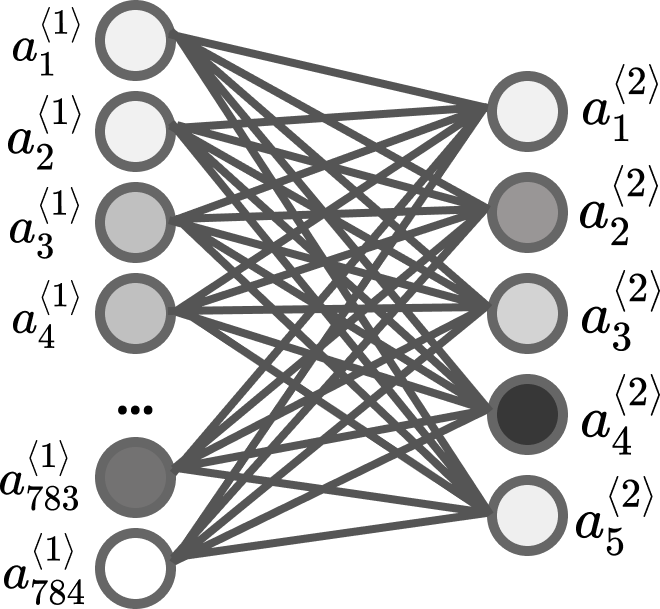
\includegraphics[width=\textwidth]{images/presentation/layer_all_all.png}
        \end{figure}
        \end{column}
        \end{columns}
    \end{frame}

    \begin{frame}{Another motivation for activation function}
        Suppose that we:
        \begin{itemize}
            \item Don't have any activation function.
            \item Neural network consists of $n_L+1$ layers with zero biases.
        \end{itemize}
        Then, based on our definition of a neural network:
        \begin{align*}
        \mathbf{a}^{\langle 2 \rangle} = \mathbf{W}^{\langle 1 \rangle}\mathbf{a}^{\langle 1 \rangle}, \\ \mathbf{a}^{\langle 3 \rangle} = \mathbf{W}^{\langle 2 \rangle}\mathbf{a}^{\langle 2 \rangle}, \\ \vdots \\ \mathbf{a}^{\langle n_L+1 \rangle} = \mathbf{W}^{\langle n_L \rangle}\mathbf{a}^{\langle n_L \rangle}.
        \end{align*}

        Therefore, $\mathbf{a}^{\langle n_L + 1 \rangle} = \mathbf{W}^{\langle n_L \rangle}\mathbf{W}^{\langle n_L-1 \rangle}\dots \mathbf{W}^{\langle 1 \rangle}\mathbf{a}^{\langle 1\rangle} = \widetilde{\mathbf{W}}\mathbf{a}^{\langle 1 \rangle}$ -- that's a \textcolor{red}{linear} dependence -- no good.
    \end{frame}

    \begin{frame}{Our architecture}
        By putting everything together, we have a complex function $f(x;\theta)$ where $\theta$ is a set of weights and biases.
    
        \begin{figure}
        \centering
            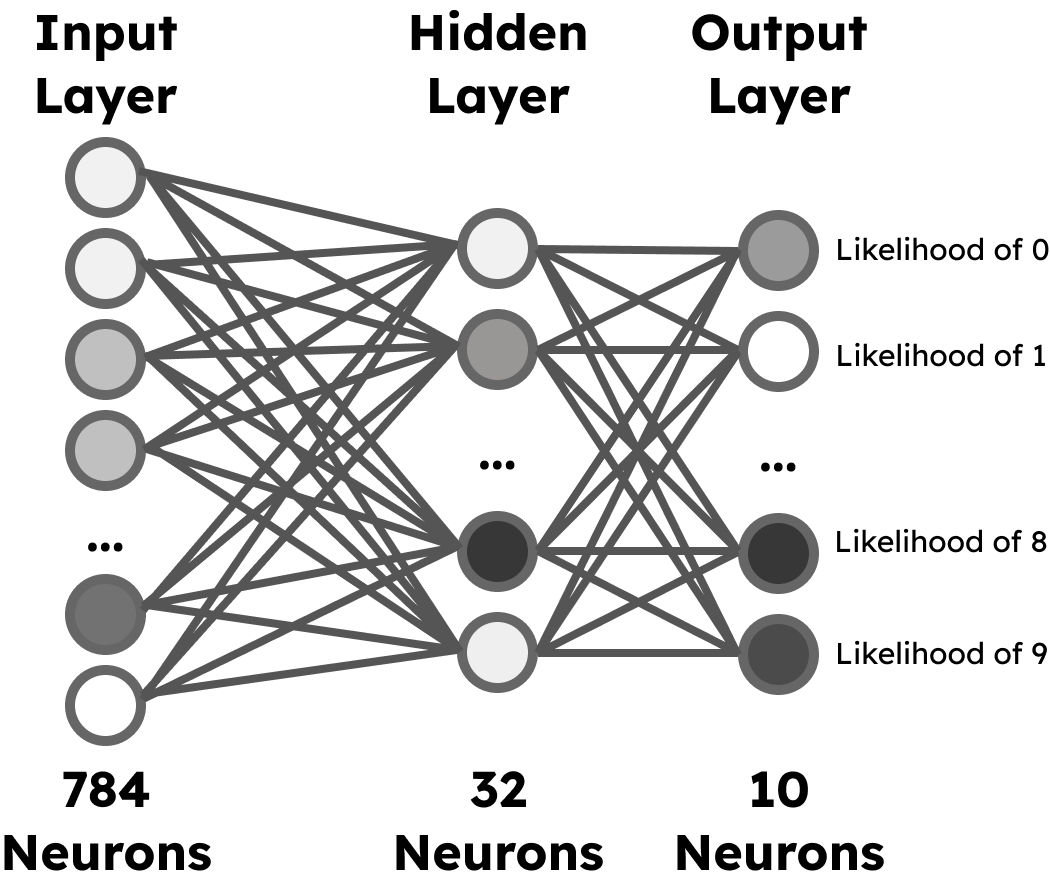
\includegraphics[width=0.57\textwidth]{images/presentation/our_architecture.png}
            \caption{Our proposed architecture for digit recognition}
        \end{figure}
    \end{frame}

    \subsection{Making neural network adjust parameters}
    \begin{frame}{Loss function motivation}
        Until this point, we haven't used dataset, so let us discuss how to apply it.
    
        \textbf{Core idea:} neural network is nothing but a HUGE parametric function $f(\mathbf{x};\theta)$ with A LOT of parameters $\theta$, which somehow outputs us a label based on input $\mathbf{x}$. 

        \begin{exampleblock}{Question}
        After inputting image of a digit $1$, you get the following output:
        \[
        [0.01, 0.05, 0.7, 0.8, 0.05, 0.3, 0.5, 0.02, 0.07, 0.03]
        \]
        Is it a good result? What about
        \[
        [0.001, 0.99, 0.01, 0.01, 0.02, 0.003, 0.1, 0.002, 0.001, 0.05]?
        \]
        \textbf{Hint:} $i^{\text{th}}$ position's value represents the likelihood of an image $i$.
        \end{exampleblock}
    \end{frame}

    \begin{frame}{Finding Ideas...}
        \begin{columns}
        \begin{column}{0.35\textwidth}
        \begin{exampleblock}{Question}
            What measure can you propose to indicate how bad the neural network performs?
        \end{exampleblock}
        \end{column}
        \begin{column}{0.65\textwidth}
        \begin{figure}
        \centering
            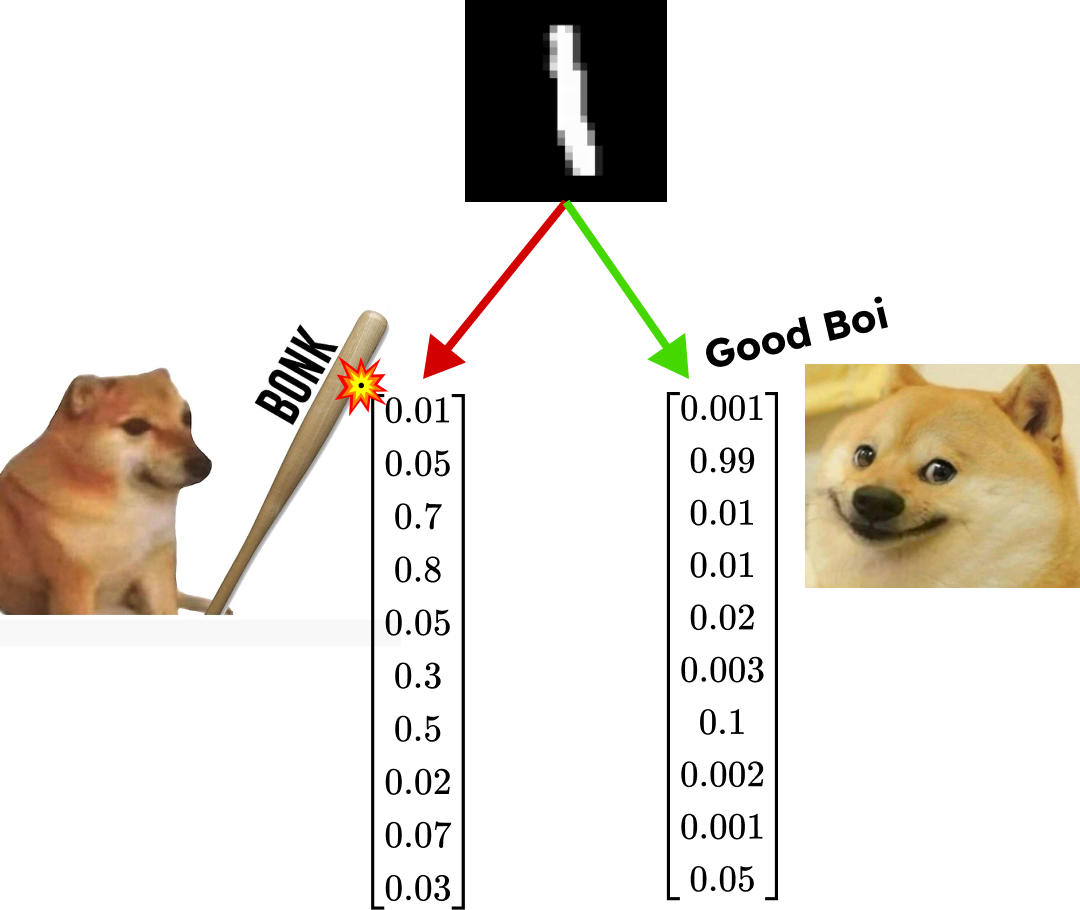
\includegraphics[width=\textwidth]{images/presentation/loss.png}
            \caption{Bad and good bois}
        \end{figure}
        \end{column}
        \end{columns}
    \end{frame}

    \begin{frame}{Mean-squared error}
        Suppose that the true label is a vector $\mathbf{y}$, where the $i^{\text{th}}$ position is $1$, if the corresponding image $\mathbf{x}$ is of digit $i$, and $0$ otherwise.

        \begin{exampleblock}{Example}
            If $\mathbf{x}$ is an image of $5$, then the corresponding label $\mathbf{y}$ is
            \[
            \mathbf{y} = [0, 0, 0, 0, 0, 1, 0, 0, 0, 0]
            \]
        \end{exampleblock}

        Ideally, we want our neural network to output $\mathbf{y}$, but it outputs $f(\mathbf{x};\theta)=\hat{\mathbf{y}}$. Define an error as $\ell(\mathbf{y},\hat{\mathbf{y}}) = \|\mathbf{y}-\hat{\mathbf{y}}\|^2=\sum_{i=1}^{10}(y_i-\hat{y}_i)^2$. Our goal is to minimize this error for all pairs of $(\mathbf{x},\mathbf{y})$ from our dataset:
        \[
        \boxed{L(\theta) = \sum_{i=1}^n \ell(\mathbf{y}_i,f(\mathbf{x}_i;\theta))}
        \]
    \end{frame}

    \begin{frame}{Interactivity!}
        \begin{block}{Question}
            Suppose we want to have a prediction $\hat{\boldsymbol{y}}$ as close as possible to the true label $\boldsymbol{y}$. Is the loss function below a good candidate? Why?
            \[
            \ell(\mathbf{y},\hat{\mathbf{y}}) = \frac{1}{\|\mathbf{y}-\hat{\mathbf{y}}\|}
            \]
        \end{block}
    \end{frame}

    \begin{frame}{What is takes to build a supervised neural network?}
        \begin{enumerate}
            \item Find the dataset: a set of inputs and desired outputs.
            \item Choose the structure: number of layers, activation functions, what is ``input'' and what is ``output''.
            \item Choose the loss function: what is considered to be a ``good'' and ``bad'' outputs.
            \item Defining training parameters: speed of learning, optimizer (we do not discuss it today).
        \end{enumerate}

        \begin{block}{Key takeaway}
            Building a neural network is nothing but specifying a function $f(X;\theta)$ with tons of parameters, feeding a list of inputs and outputs, and finding such parameters $\hat{\theta}$, which minimizes the error on the given dataset.
        \end{block}
    \end{frame}

    \section{Coding Time!}

    \subsection{Tools}

    \begin{frame}{Tools for Deep Learning / Machine Learning}
        \begin{figure}
        \centering
            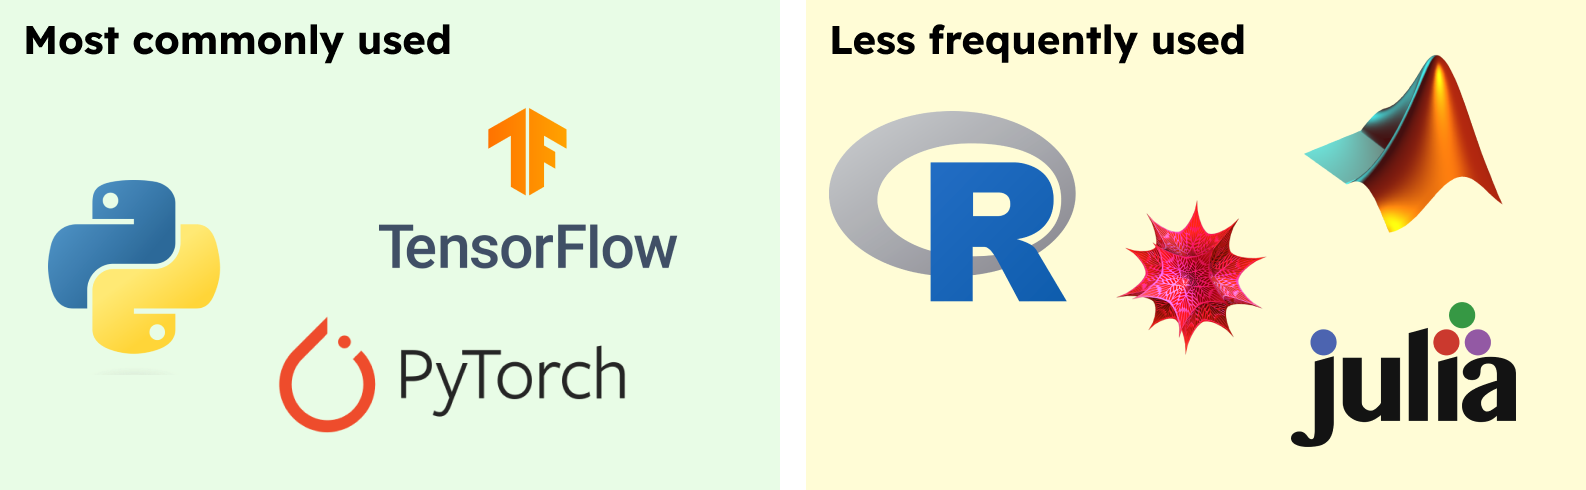
\includegraphics[width=\textwidth]{images/presentation/tools.png}
            \caption{Tools used for Deep and Machine Learning}
        \end{figure}
    \end{frame}

     \begin{frame}{A Neural Network Playground}
        \begin{figure}
        \centering
            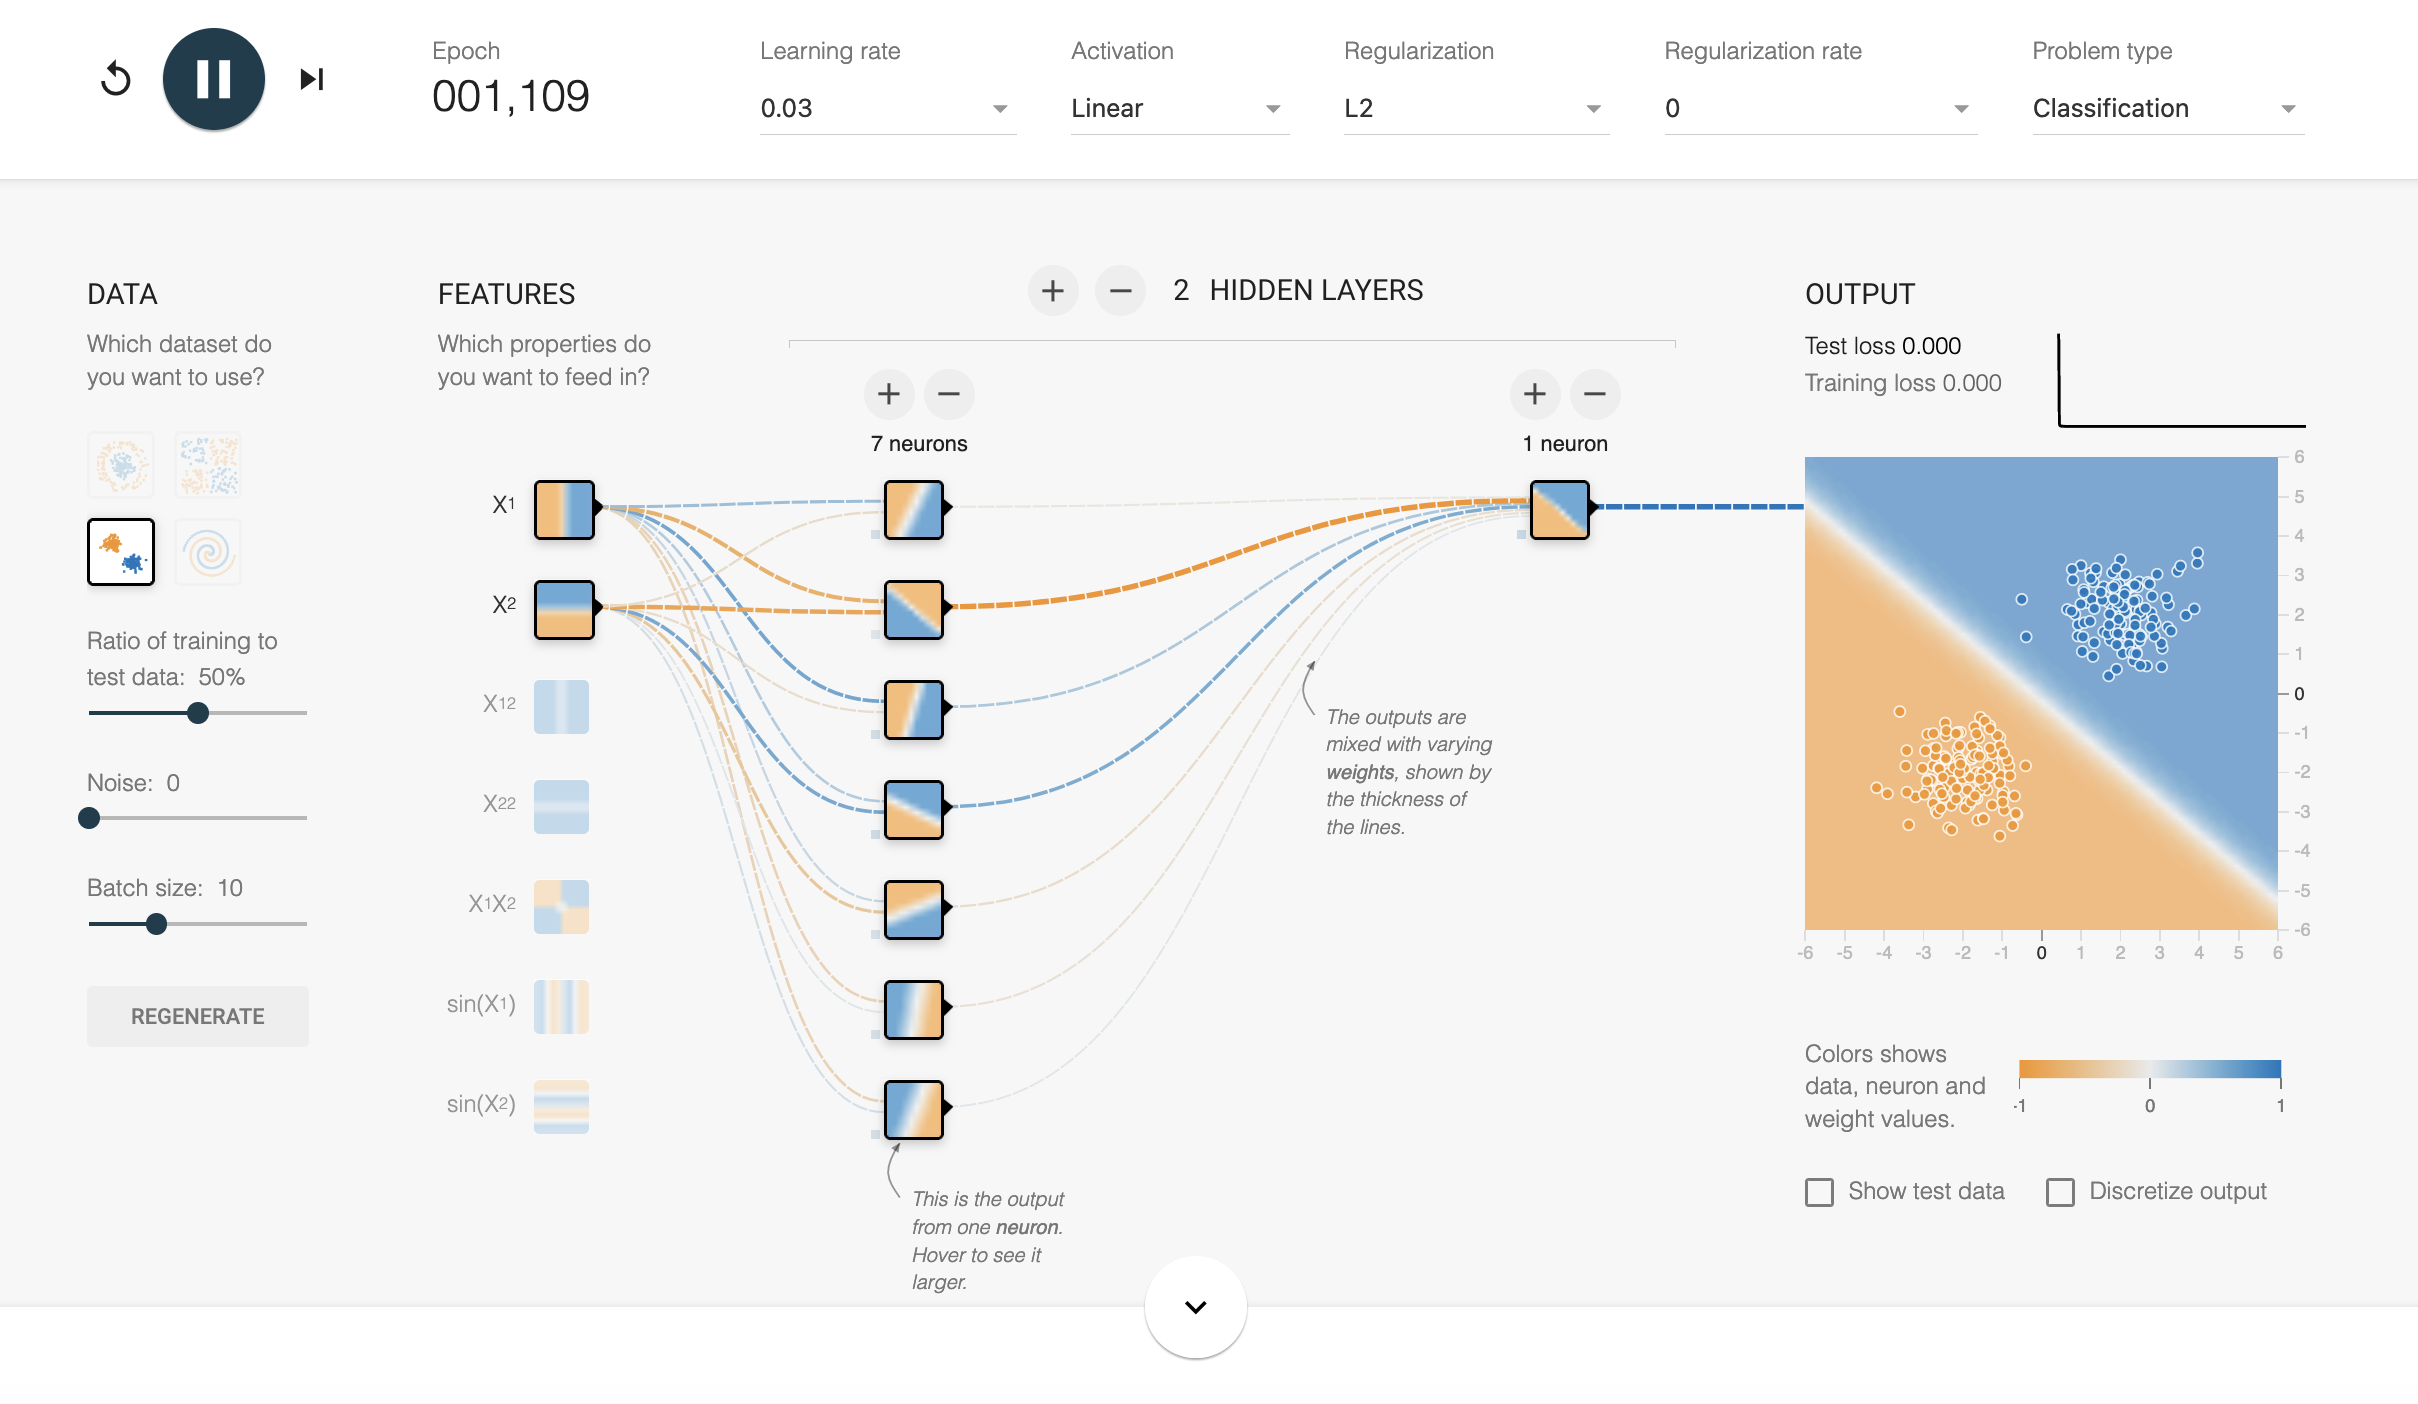
\includegraphics[width=\textwidth]{images/presentation/playground.png}
            \caption{Tensorflow Playground. See \href{https://playground.tensorflow.org}{https://playground.tensorflow.org}}
        \end{figure}
    \end{frame}

    \subsection{Solution using Tensorflow}
    \begin{frame}[fragile]{Importing packages}
        \begin{lstlisting}[language=Python, caption=Importing packages we would use]
import tensorflow as tf # For defining and training the neural network
import numpy as np # For convenient use of high-dimensional arrays
from keras import datasets # For loading the MNIST dataset

print(f'Using TensorFlow {tf.__version__}')
np.set_printoptions(precision=3)
        \end{lstlisting}
    
    \end{frame}

    \begin{frame}[fragile]{Importing MNIST dataset}
        \begin{lstlisting}[language=Python, caption=Importing the MNIST dataset]
(X, y), _ = datasets.mnist.load_data()
X = X / 255.0
y = np.array([[1.0 if i == label else 0.0 for i in range(10)] for label in y])
        \end{lstlisting}
    
    \end{frame}

    \begin{frame}[fragile]{Defining the neural network structure}
        \begin{lstlisting}[language=Python, caption=Defining the neural network structure]
neural_network = tf.keras.models.Sequential([
    tf.keras.layers.Flatten(input_shape=(28,28)),
    tf.keras.layers.Dense(
        32,
        name='hidden_layer',
        activation='sigmoid'
    ),
    tf.keras.layers.Dense(
        10,  
        name='output_layer',
        activation='sigmoid'
    )
])
        \end{lstlisting}
    
    \end{frame}

    \begin{frame}[fragile]{Fitting into the neural network}
        \begin{lstlisting}[language=Python, caption=Launch the training session]
optimizer = tf.keras.optimizers.legacy.Adam(learning_rate=1e-5)
neural_network.compile(loss='mse', optimizer=optimizer)
neural_network.fit(
    X, 
    y,
    epochs=30,
    verbose=1,
    validation_split=0.2
)
        \end{lstlisting}
    \end{frame}

    \begin{frame}[fragile]{Testing!}
            \begin{lstlisting}[language=Python, caption=Launch the testing]
# Making prediction
index = 1 # Put your index to test
prediction = neural_network.predict(np.expand_dims(X[index], axis=0), verbose=0)

# Displaying results
print(f'Prediction in raw format: {prediction}')
show_image(X[index], np.argmax(prediction[0]))
    \end{lstlisting}
    \end{frame}
    
	\begin{frame}{}
      \centering \Large
      \emph{Thank you for your attention!}
    \end{frame}

\end{document}